\documentclass[a4paper,12pt]{article}
\usepackage[utf8]{inputenc}
\usepackage[T1]{fontenc}
\usepackage{svg}
\usepackage{mathtools}
\usepackage{graphicx} 
\usepackage{float}
\usepackage{here}
\usepackage{xcolor}
\usepackage{listings}
\usepackage{amsmath}
\usepackage{booktabs} % For pretty tables
\usepackage[center]{caption} % For caption spacing
\usepackage{subcaption} % For sub-figures
\usepackage{graphicx}
\usepackage[all]{nowidow}
\usepackage[utf8]{inputenc}
\usepackage{tikz}
\usepackage{multicol}
\usepackage{algpseudocode,algorithm,algorithmicx}
\usepackage{cases}
\usepackage{minted}
\usepackage[affil-it]{authblk}
\usepackage{booktabs}
\usepackage[inline]{enumitem} 
\usepackage[nottoc]{tocbibind}
\usepackage[colorlinks=true, linkcolor=blue, citecolor=blue, urlcolor=blue, breaklinks=true]{hyperref}
\usepackage{microtype} 
\providecommand{\keywords}[1]
{
  \small	
  \textbf{Keywords ---} #1
}
\newcommand{\fact}[1]{#1\mathpunct{}!}


\DeclareCaptionType{equ}[][]
\makeatletter
\lstnewenvironment{code}[1][]
    {\lstset{language=haskell,
    basicstyle=\small\ttfamily,
    numbers=left,
    numberstyle=\tiny\color{gray},
    backgroundcolor=\color{lightgray},
    firstnumber=auto,
    name=main,
    #1}%
    \csname\@lst @SetFirstNumber\endcsname}
    {\csname\@lst @SaveFirstNumber\endcsname}
\makeatother
\title{Spectral separation of the stochastic background for LISA and study of the separability of the cosmological background level $\Omega_0$}
\author{Guillaume BOILEAU}
\affil{Laboratoire Artemis UMR - 7250 Electronic~address:~\texttt{guillaume.boileau@oca.eu}}
\date{\today}

\begin{document}

\maketitle
\begin{abstract}
In the context of the attempt to observe the stochastic gravitational wave background with LISA, the study of the spectral separability of the Cosmological and Astrophysical is important to estimated the cosmological background level. We need to fix some limits for this attempted measurement of the Stochastic Gravitational Wave Backgrounds (SGWB). We develop Adaptive Markov chains Monte-Carlo (Adaptive-McMC) to estimated simulated data from the LISA Data challenge (LDC). We also develop Fisher matrix Information of the Whittle Likelihood to estimate the uncertainty   
\end{abstract}

\keywords{Spectral separability, Stochastic Gravitational Wave Background, LISA, Adaptive Markov chains Monte-Carlo, Fisher matrix Information, Whittle Likelihood.}

\section{Introduction}
In this document, we will introduce the Fisher analysis performed for the spectral separation of Neil Cornish (Section~\ref{spectral}: Spectral Separation). And then realized the study of the measurement of $\Omega_0$ for the stochastic background of LISA. We also present a study of the Adaptive McMC , a method to fit the parameters of the stochastic backgrounds. We introduce the MLDC Data for a treatment with the Adaptive McMC algorithm.

\section{Spectral Separation \label{spectral}}
A useful toy model to consider is the problem of separating two independent Gaussian noise processes that have different power spectra. Suppose we have data that is formed from the sum of two independent noise processes. In the frequency domain we can write:

\begin{equation}
    d(f) = n_1(f) +n_2(f)
\end{equation}

Let us assume that both processes have zero mean : 

\begin{equation}
    E[n_1(f)] = 0 \hspace{1cm}  E[n_2 (f )] = 0 ,
\end{equation}

and the power spectra :

\begin{equation}
    E[n_1(f)n_1^{\star}(f')] = S_{n_1}(f)\delta_{ff'}
\end{equation}
with $S_{n_1} = A_1f^{\alpha_1}$ and similarly for $n_2$. Our assumption of independence implies that the cross
spectra vanish: $E[n_1(f)n_2^{\star} (f')] = 0$. The data $d$ are measured across the frequency band $[f_a , f_b ]$,
which for a finite observation time $T$ corresponds to having samples between bins $a = f_a T$ and
$b = f_b T$ . The Whittle likelihood can be written:

\begin{equation} \label{likelihood}
    p(d|A_1 , \alpha_1 , A_2 , \alpha_2) = \prod_{k=a}^b \frac{1}{\sqrt{S(f_k)}} e^{-\frac{d^{\star}(f_k) d(f_k)}{2 S(f_k)}}
\end{equation}

where $S(f_k ) = A_1f_k^{\alpha_1} + A_2f_k^{\alpha_2}$ . While real data will have discrete frequency samples, the calculation can be simplified by treating the frequencies as continuous. The product $d^{\star}(f_k) d(f_k)$ is the real part of the Fourier transform of the Times-series at the frequency $f_k$, we use the Energy spectral density. This product is a sum of the two power law.  The  log likelihood can be approximated as

\begin{equation}
    \ln p(d|A_1 , \alpha_1 , A_2 , \alpha_2) = -\frac{1}{2} \int_{f_a}^{f_b} \left( \frac{d^{\star}(f) d(f)}{S(f)} + \ln S(f) \right) df 
\end{equation}

The log likelihood can be write as, with the expected value of the sum of powers spectra $E[S(f)] =
A_1f^{\alpha_1}+A_2f^{\alpha_2}$ and the expected value of the cross Fourier
transform can be write $E[d^{\star}(f)d(f)] = \overline{A_1}f^{\overline{\alpha_1}} +
\overline{A_2}f^{\overline{\alpha_2}}$ (We assume the parameter $(A_1 , \alpha_1 , A_2 , \alpha_2 )$
and ($\overline{A_1} , \overline{\alpha_1} , \overline{A_2} , \overline{\alpha_2})$ are independent)~:

\begin{equation}
    \ln p(d|A_1 , \alpha_1 , A_2 , \alpha_2) = -\frac{1}{2} \int_{f_a}^{f_b} \left( \frac{\overline{A_1}f^{\overline{\alpha_1}} + \overline{A_2}f^{\overline{\alpha_2}}}{A_1f^{\alpha_1} + A_2f^{\alpha_2}} + \ln (A_1f^{\alpha_1} + A_2f^{\alpha_2}) \right) df 
\end{equation}
Here the barred quantities denote the true values. We assume Writing the parameter vector as $\overrightarrow{\lambda} \to (A_1 , \alpha_1 , A_2 , \alpha_2 )$, the maximum likelihood solution is found by solving the set of equations $\partial_i \ln \ p(d|\overrightarrow{\lambda}) = 0$ where we are using the notation $\partial_i = \partial/\partial \lambda_i$ . Consider for now the derivative with respect to $A_1$ , which yields the condition

\begin{equation}
    \int_{f_a}^{f_b} \left( \frac{(\overline{A_1}f^{\overline{\alpha_1}} + \overline{A_2}f^{\overline{\alpha_2}}) + (A_1f^{\alpha_1} + A_2f^{\alpha_2}) }{(A_1f^{\alpha_1} + A_2f^{\alpha_2})^2} \right) df = 0
\end{equation}

The only non-trivial solution that is valid for any choice of integration interval has $\overline{A_1} = A_1 , \overline{\alpha_1} = \alpha_1, \overline{A_2} = A_2 , \overline{\alpha_2} = \alpha_2$ . 

\subsection{The Fisher information}
The Fisher information matrix is given by the negative Hessian of the
expected log likelihood evaluated at maximum-likelihood:

\begin{equation}
    \Gamma_{i,j} = -E[\partial_i \partial_j \ln p(d|A_1,A_2,\alpha_1,\alpha_2)]  \label{Fisher}
\end{equation}

We can introduce an preliminary quantity to calculated the Fisher Information, $\gamma_{ij}$ where $\Gamma_{ij} = E[\gamma_{ij}]$. The next equation \ref{eq:gamma11} to \ref{eq:gamma43}, correspond to the first part of the calculation of the Fisher Information matrix $\Gamma_{ij}$ :

\begin{equation}\label{eq:gamma11}
    \gamma_{11} =  \int_{f_a}^{f_b} \frac{ f^{2 \overline{ \alpha_1}}}{2(\overline{A_1}f^{\overline{ \alpha_1}} +\overline{A_2}f^{\overline{ \alpha_2}})^2} \, \mathrm{d}f 
\end{equation}

\begin{equation}
    \gamma_{22} = \int_{f_a}^{f_b} \frac{ (\overline{A_1}f^{\overline{ \alpha_1}} \ln f )^2}{2(\overline{A_1}f^{\overline{ \alpha_1}} +\overline{A_2}f^{\overline{ \alpha_2}})^2} \, \mathrm{d}f 
\end{equation}

\begin{equation}\label{eq:gamma33}
    \gamma_{33} =  \int_{f_a}^{f_b} \frac{ f^{2 \overline{ \alpha_2}}}{2(\overline{A_1}f^{\overline{ \alpha_1}} +\overline{A_2}f^{\overline{ \alpha_2}})^2} \, \mathrm{d}f 
\end{equation}

\begin{equation}
    \gamma_{44} = \int_{f_a}^{f_b} \frac{ (\overline{A_2}f^{\overline{ \alpha_2}} \ln f )^2}{2(\overline{A_1}f^{\overline{ \alpha_1}} +\overline{A_2}f^{\overline{ \alpha_2}})^2} \, \mathrm{d}f 
\end{equation}

\begin{equation}
    \gamma_{12} =  \int_{f_a}^{f_b} \frac{\overline{A_1}f^{2 \overline{ \alpha_1}} \ln f}{2(\overline{A_1}f^{\overline{ \alpha_1}} +\overline{A_2}f^{\overline{ \alpha_2}})^2} \, \mathrm{d}f 
\end{equation}

\begin{equation}
    \gamma_{13} =  \int_{f_a}^{f_b} \frac{f^{\overline{ \alpha_1}+\overline{ \alpha_2}} }{2(\overline{A_1}f^{\overline{ \alpha_1}} +\overline{A_2}f^{\overline{ \alpha_2}})^2} \, \mathrm{d}f 
\end{equation}

\begin{equation}
    \gamma_{14} =  \int_{f_a}^{f_b} \frac{ \overline{A_2} f^{\overline{ \alpha_1} + \overline{ \alpha_2}} \ln f }{2(\overline{A_1}f^{\overline{ \alpha_1}} +\overline{A_2}f^{\overline{ \alpha_2}})^2} \, \mathrm{d}f 
\end{equation}

\begin{equation}
    \gamma_{21} =  \int_{f_a}^{f_b} \frac{ \overline{A_1} f^{\overline{2 \alpha}_1}  \ln f}{2(\overline{A_1}f^{\overline{ \alpha_1}} +\overline{A_2}f^{\overline{ \alpha_2}})^2} \, \mathrm{d}f 
\end{equation}

\begin{equation}
    \gamma_{23} =  \int_{f_a}^{f_b} \frac{ \overline{A_1} f^{\overline{ \alpha}_1 + \overline{ \alpha}_2}  \ln f}{2(\overline{A_1}f^{\overline{ \alpha_1}} +\overline{A_2}f^{\overline{ \alpha_2}})^2} \, \mathrm{d}f 
\end{equation}

\begin{equation}
    \gamma_{24} =  \int_{f_a}^{f_b} \frac{ \overline{A_1} \overline{A_2} f^{\overline{ \alpha}_1 + \overline{ \alpha}_2}  \ln ^2 f}{2(\overline{A_1}f^{\overline{ \alpha_1}} +\overline{A_2}f^{\overline{ \alpha_2}})^2} \, \mathrm{d}f 
\end{equation}


\begin{equation}
    \gamma_{31} =  \int_{f_a}^{f_b} \frac{ f^{\overline{ \alpha}_1 + \overline{ \alpha}_2}}{2(\overline{A_1}f^{\overline{ \alpha_1}} +\overline{A_2}f^{\overline{ \alpha_2}})^2} \, \mathrm{d}f 
\end{equation}

\begin{equation}
    \gamma_{32} =  \int_{f_a}^{f_b} \frac{ \overline{A_1} f^{\overline{ \alpha}_1 + \overline{ \alpha}_2}  \ln f}{2(\overline{A_1}f^{\overline{ \alpha_1}} +\overline{A_2}f^{\overline{ \alpha_2}})^2} \, \mathrm{d}f 
\end{equation}

\begin{equation}
    \gamma_{34} =  \int_{f_a}^{f_b} \frac{\overline{A_2}f^{2 \overline{ \alpha_2}} \ln f}{2(\overline{A_1}f^{\overline{ \alpha_1}} +\overline{A_2}f^{\overline{ \alpha_2}})^2} \, \mathrm{d}f 
\end{equation}

\begin{equation}
    \gamma_{41} =  \int_{f_a}^{f_b} \frac{ \overline{A_2} f^{\overline{ \alpha}_1 + \overline{ \alpha}_2}  \ln f}{2(\overline{A_1}f^{\overline{ \alpha_1}} + \overline{A_2}f^{\overline{ \alpha_2}})^2} \, \mathrm{d}f 
\end{equation}

\begin{equation}
    \gamma_{42} =  \int_{f_a}^{f_b} \frac{ \overline{A_1} \overline{A_2} f^{\overline{ \alpha}_1 + \overline{ \alpha}_2}  \ln ^2 f}{2(\overline{A_1}f^{\overline{ \alpha_1}} +\overline{A_2}f^{\overline{ \alpha_2}})^2} \, \mathrm{d}f 
\end{equation}

\begin{equation}\label{eq:gamma43}
    \gamma_{43} =  \int_{f_a}^{f_b} \frac{ \overline{A_2} f^{\overline{2 \alpha}_2}  \ln f}{2(\overline{A_1}f^{\overline{ \alpha_1}} +\overline{A_2}f^{\overline{ \alpha_2}})^2} \, \mathrm{d}f 
\end{equation}

Now, when $\alpha_1 = \alpha_2$ we have $\Gamma_{22} = \overline{A_1}^2 I, \Gamma_{44} = \overline{A_2}^2 I, \Gamma_{24} = \overline{A_1} \overline{A_2} I$ where 

\begin{equation}
    I = \int_{f_a}^{f_b} \frac{(\ln f)^2 (f^{\overline{\alpha_1}})^2}{2 (\overline{A_1}f^{\overline{ \alpha_1}} +\overline{A_2}f^{\overline{ \alpha_2}})^2}
\end{equation}

We can write an integral to summarize the sixteen integral, we can use ($ a $, $ b $, $ c $) the three slopes of the three numerator's component  ($\overline{A_1}f^{\overline{\alpha_1}}$,$\overline{A_2}f^{\overline{\alpha_2}}$,$ln(f)$). It is thus easier to describe the integrals according to the powers ($ a $, $ b $, $ c $), indeed for example the integral $\Gamma_{24}$ is ($ a= 1 $, $ b = 1 $, $ c =2 $). However, for certain integrals, we need to multiply by a factor depending on $\overline{A_1}$ and $\overline{A_2}$. The table~\ref{Table:Inte} summarize the conversion between $I(a,b,c)$ and $\Gamma_{i,j}$. We need to calculate this integral:

\begin{equation}
    I(a,b,c) = \int_{f_a}^{f_b} \frac{{\left(\overline{A_1}f^{\overline{\alpha_1}}\right)}^a {\left(\overline{A_2}f^{\overline{\alpha_2}}\right)}^b}{2(\overline{A_1}f^{\overline{ \alpha_1}} +\overline{A_2}f^{\overline{ \alpha_2}})^2}  \ln^c(f) \mathrm{d}f
\end{equation}

It is easier to write : 

\begin{equation}
    I(a,b,c) = D \int_{f_a}^{f_b} \frac{f^{a \overline{ \alpha_1} + \overline{ \alpha_2}(b-2)}}{\left(1 + \frac{\overline{A_1}}{\overline{A_1}} f^{\overline{ \alpha_2} - \overline{ \alpha_1}}\right)^2} \ln^c(f) \mathrm{d}f
\end{equation}

We use $f = e^u$,

\begin{equation}
    I(a,b,c) = D \int_{\ln f_a}^{\ln f_b} \frac{e^{uA}u^c}{(1+Ce^{uB})^2} \mathrm{d}u
\end{equation}
 with $A = a \overline{ \alpha_2} + \overline{ \alpha_1}(b-2)+1 $, $B=\overline{ \alpha_2} -\overline{ \alpha_1}$, $C = \frac{\overline{A_2}}{\overline{A_1}}$ and $D = \frac{\overline{A_2}^a \overline{A_1}^{b-2}}{2}$.
 
 We can calculated the integral $I_c$ for the three values of $c$: 
 \begin{itemize}
     \item c = 0 
 \end{itemize}

        \begin{equation}
            I(a,b,0) = D \left[ \frac{e^{Au}}{A} {}_2F_1 \left(2, \frac{A}{B}; \frac{A+B}{B}; -Ce^{Bu} \right) \right]_{\ln f_a}^{\ln f_b}
        \end{equation}

 \begin{itemize}        
     \item c = 1
 \end{itemize}
 
\begin{equation}
        \begin{split}
        I(a,b,1)&= D \Bigg [ \frac{e^{Au}}{A^2} \Bigg({}_2F_1 \left(2, \frac{A}{B}; \frac{A+B}{B}; -Ce^{Bu} \right)\\[.5em]
        &- {}_3F_2 \left(2, \frac{A}{B}, \frac{A}{B}; \frac{A+B}{B}, \frac{A+B}{B}; -Ce^{Bu} \right) \Bigg) \Bigg]_{\ln f_a}^{\ln f_b}
        \end{split}
\end{equation}
\begin{itemize}
     \item c = 2 
    \end{itemize}       
          
        \begin{equation}
            \begin{split}
                I(a,b,2)&= D \Bigg [ \frac{e^{Au}}{A^3 B} \Bigg(2 A(u(A-B)+1) {}_3F_2 \left( 1, \frac{A}{B}, \frac{A}{B}; \frac{A+B}{B}, \frac{A+B}{B}; -C e^{Bu} \right)\\[.5em]
                &+2(B-A) {}_4F_3 \left( 1, \frac{A}{B}, \frac{A}{B}, \frac{A}{B}; \frac{A+B}{B},\frac{A+B}{B}, \frac{A+B}{B}; -C e^{Bu} \right)\\[.5em]
                &+ A^2u ((B-A)u -2)(Ce^{Bu}+1){}_2F_1 \left(1, \frac{A}{B}; \frac{A+B}{B}; -Ce^{Bu} \right)\Bigg) \Bigg]_{\ln f_a}^{\ln f_b}   
            \end{split}
        \end{equation}

 with ${}_pF_q\left(a_1, ..., a_p; b_1,... , b_q;x\right) = \sum_{n=0}^\infty \frac{(a_1)_n ... (a_p)_n}{(b_1)_n ... (b_q)_n}\frac{x^n}{\fact{n}}$ the generalize hypergeometric function and $(\alpha)_j = \alpha(\alpha+1)...(\alpha+i-1)$ the  Pochhammer symbol. 



\begin{table}[H]
\begin{center}
\begin{tabular}{|l|l|l|l|}
\hline
$\mathbf{\Gamma_{ij}}$    & $\mathbf{I(a,b,c)}$                                      & $\mathbf{\Gamma_{ij}}$    & $\mathbf{I(a,b,c)}$                        \\ \hline
$\Gamma_{11}$             & $\left(\overline{A_1}\right)^{-2}I(2,0,0)$               & $\Gamma_{23}=\Gamma_{32}$ & $\left(\overline{A_2}\right)^{-1}I(1,1,1)$ \\ \hline
$\Gamma_{12}=\Gamma_{21}$ & $\left(\overline{A_1}\right)^{-1}I(2,0,1)$               & $\Gamma_{24}=\Gamma_{42}$ & $I(1,1,2)$                                 \\ \hline
$\Gamma_{13}=\Gamma_{31}$ & $\left(\overline{A_1}\overline{A_1}\right)^{-1}I(1,1,0)$ & $\Gamma_{33}$             & $\left(\overline{A_2}\right)^{-2}I(0,2,0)$ \\ \hline
$\Gamma_{14}=\Gamma_{41}$ & $\left(\overline{A_1}\right)^{-1}I(1,1,1)$               & $\Gamma_{34}=\Gamma_{43}$ & $\left(\overline{A_2}\right)^{-1}I(0,2,1)$ \\ \hline
$\Gamma_{22}$             & $I(2,0,2)$                                               & $\Gamma_{44}$             & $I(0,2,2)$                                 \\ \hline
\end{tabular}
\end{center}
\caption{Conversion between $I(a,b,c)$ and $\Gamma_{i,j}$}
\label{Table:Inte}
\end{table}

\subsection{The Cramer-Rao bound}\label{sec:Cramer}

For parameters  $ \widehat{\theta}$, we can write the Fisher Information matrix as :
\begin{equation}
    \mathcal{I}(\widehat{\theta}) = E\left[-\frac{\partial}{\partial \theta_i}\frac{\partial}{\partial \theta_j} \ln{p(d|\widehat{\theta})}\right]
\end{equation}
We can estimate the lower bound on the variance of an unbiased estimator, this is the lower bound of the Cramér-Rao. 
\begin{equation}
    {\sigma_{\widehat{\theta}}}^2 \ge \mathcal{I}(\widehat{\theta})^{-1} = \frac{1}{E\left[-\frac{\partial}{\partial \theta_i}\frac{\partial}{\partial \theta_j} \ln{p(d|\widehat{\theta})}\right]}
\end{equation}



\section{Calculation and Computing}

In this part, I follow the original Neil's paper (spectral Separation). The goal of this part is to introduce and explain me code allow with this document. All my code are codding with the Python3.6.6. 

\subsection{Fisher Information matrix}\label{study1}
he
For the computing of the Fisher information matrix, I use the definition from the equation \ref{Fisher}. For the integration, we use the LISA frequency band $f_a = 1. \ 10^{-5} \ \text{Hz}$ to $f_b = 1 \ \text{Hz}$. This is the LISA frequency band of measurements. 

We need to calculated numerically the $\gamma_{ij}$ integral \ref{eq:gamma11} to \ref{eq:gamma43} in the LISA frequency band [$f_a$, $f_b$]. This segment includes several orders of magnitude. In order not to favor the highest magnitude, we choose to integrate according to a logarithmic vector normalize by the frequency reference $f_* = 25 \text{ Hz}$ . Thus, the trapezium algorithm (Equation~\ref{eq:trapeze}) can be used before this logarithmic vector. We can therefore introduce a number $N$ of values into this vector. In the figure \ref{fig:gamma33}, this is the integral \ref{eq:gamma33} with different values of $N$ (10, 20, 50, 100, 200, 300, 400, 500, 100, 2000). According to the figure \ref{fig:gamma33}, the numerical integration seems to converge. In the rest of the document, we use $N = 1000$. 

\begin{equation}\label{eq:trapeze}
    I_N = \sum_{k=1}^{N} \frac{f(x_{k-1})  f(x_{k})}{2} (x_k-x_{k-1})
\end{equation}
with $x$ in the logarithmic vector normalize by the frequency reference $f_* = 25 \text{ Hz}$.

We can also calculate the Fisher Information with a discrete sum, for example if we considerate the
factor $\gamma_{33}$ we can write :

\begin{equation}\label{eq:sum_discrete}
    \gamma_{33} = \frac{1}{2} \sum_k \frac{ {f_k}^{2 \overline{ \alpha_2}}}{2(\overline{A_1}{f_k}^{\overline{ \alpha_1}} +\overline{A_2}{f_k}^{\overline{ \alpha_2}})^2}
\end{equation}   

On the figure \ref{fig:gamma33}, we add a black scatter plot as the discrete calculation from the equation \ref{eq:sum_discrete}. The discrete and the continues integration of the elements $\gamma_{33}$ are similar.    

\begin{figure}[H]
    \centering
    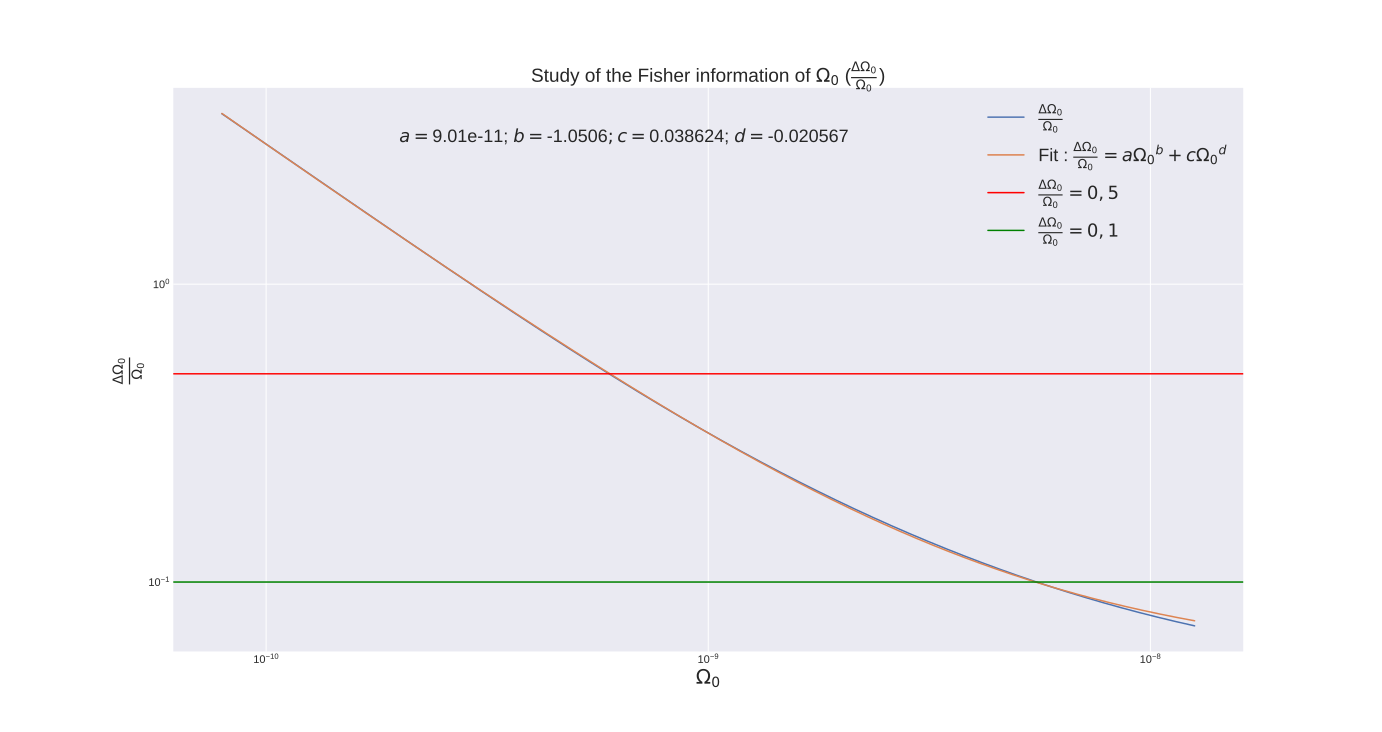
\includegraphics[height= 5.5cm]{Fisher.png}
    \caption{Convergence test of the integration of $\gamma_{33}$ \ref{eq:gamma33} with a logarithmic vector normalized by the reference frequency $f_* = 25 \text{ Hz}$. The different values of $N$ correspond to the number of elements in the vector.}
    \label{fig:gamma33}
\end{figure}

The expected value can be calculated using Gaussian distributions around the parameters to be estimated. We generate for the four parameters a normal distribution locate for to the true value of the parameters and with a rate $\frac{\sigma_{\theta_i}}{\mu_{\theta_i}} = 0.1$. According to the equation~\ref{eq:expect}, the expected value of the preliminary quantity $\gamma_{ij}$ is the mean of the sample of the preliminary quantity $\gamma_{ij}$ evaluated following independent normal distributions. 

\begin{equation}\label{eq:expect}
    E\left[\gamma_{ij}\right] = \overline{\gamma_{ij}\left(\widehat{\Theta}\right)}
\end{equation}
with $\Theta_i \hookrightarrow \mathcal{N}(\mu_{\theta_i},\sigma_{\theta_i})$, we randomly draw a sample of 100 elements from each distribution.
 
We thus obtain, by combining the numerical computation of the integrals $\gamma_{ij}$ (see equation \ref{eq:trapeze})with the trapezoid method and the estimation of the expected value (see equation \ref{eq:expect}) with normal distributions around the "true" values, an estimate of Fisher Information Matrix.

\subsection{The Cramer-Rao bound and Uncertainty}

According to the section \ref{sec:Cramer}, the standard deviation of a parameters $\widehat{\theta}$ is given by the square root of the inverse of the diagonal Fisher Information matrix $ \sigma_{\theta_{i}} = \frac{1}{\Gamma_{ii}}$. It is a maximization of the standard deviation$ \sigma_{\theta_{i}}$. We can take this value of the estimation of the separability. The inverse of the Fisher Information Matrix is the covariance matrix. 

\begin{equation}
    {Cov}^{ij} = (\Gamma^{-1})^{ij} = E[\Delta\theta^i \Delta \theta^j]
\end{equation}

On the diagonal we have ${Cov}^{ii} = \sigma_i^2$


The purpose of this study is to calculate with Fisher's information study the uncertainty of $\theta_i$ $\frac{\Delta \theta_i}{\theta_i}$. This study makes it possible to have a threshold of separability by a Adaptive McMC with the likelihood of the equation~ \ref{likelihood}. In the next of our study We will thus have a limit value of separability of the cosmological parameter and the astrophysical backgound. If the uncertainty of a parameters $\theta_i$ is equal to $0.1$, we measure the parameters with on error of $10\%$.

The uncertainty of $\theta_i$ is given by : 

\begin{equation}
    \frac{\Delta \theta_i}{\theta_i} = \frac{\sqrt{Cov^{ii}}}{\theta_i} \le \frac{1}{\theta_i}\sqrt{\frac{1}{ E\left[-\frac{\partial}{\partial \theta_i}\frac{\partial}{\partial \theta_i} \ln{p(d|\widehat{\theta})}\right]}} 
\end{equation}


 \section{Markov chains Monte-Carlo Adaptive (McMC-Adaptive)} \label{sc:adap_McMC}
\subsection{Markov chains Monte-Carlo (McMC)}
Bayesian inference is an inference method by which the probabilities of various hypothetical causes are calculated from the observation of known events. It is based on the Bayes theorem (see equation~ \ref{eq:bayes}). 

The goal of a Bayes study is to know the posterior distribution, but we do not have access to this distribution, but we have access to the likelihood distribution. We can model the data $d$ with a model $m$. Thus, it is possible to estimate the posterior distribution by looking at the distribution of a sample of parameter modeling product. There are strategies for choosing parameters and estimating posterior distribution. The Markov chains Monte Carlo is an numerical strategy to fit parameters from DATA. 
This is a sampling method using distribution of probability. The McMC method consists to  draw random samples of a multidimensional parameter $x$ (parameter of the model $m$). We use a probability density distribution $\pi(x)$ to use probability distributions. Comparison of a random draw of a model parameter with data.

\begin{equation}\label{eq:bayes}
    p(m|d) = \frac{p(d|m)}{p(m)}p(d)
\end{equation}
where $p(d)$ is the prior distribution, $p(m|d)$ is the posterior distribution, $p(d|m)$ is the likelihood distribution and $p(m)$ is the evidence of the model distribution. 
\subsection{Metropolis-Hasting sampler}
Monte Carlo methods by Markov chains (MCMC) are based on the simulation of a Markov chain (Random and iterative drawing of
independent parameter). There are as many chains as parameters to estimate, in our case 4. To generate chains we can use the
Metropolis-Hastings algorithm. This is based on the rejection or acceptance of parameters according to the likelihood ratio
between two neighboring parameters. Thus, the parameters maximizing the likelihood are favored. Indeed, the likelihood is
maximum when the model best describes the data. \newline

\textbf{Metropolis-Hastings algorithm}
    \begin{itemize}
        \item initial point (star) $x_0$ and chose a prior function $P(x)$. 
        \item at the i-th iteration:
            \begin{itemize}
                \item Generation of the candidate $x'$ with the distribution $g(x'|x_i)$ (Gaussian)
                \item Calculation
                    \begin{itemize}
                        \item likelihood of $x_i$ and $x'$, $p(d|m(x_i))$ and $p(d|m(x'))$
                        \item prior of $x_i$ and $x'$, $P(x')$ and $P(x_i)$
                        \item ratio $\alpha = \frac{p(d|m(x'))}{p(d|m(x_i))} \frac{P(x')}{P(x_i)}$
                    \end{itemize}
                \item Accept/Reject
                \begin{itemize}
                    \item Generation of a uniform random number $u$ on $[0,1]$
                    \item if $u \leq \alpha$, accept the candidate : $\alpha_{i+1} = x'$
                    \item if $u > \alpha$, reject the candidate : $x_{i+1} = x_i$
                \end{itemize}
            \end{itemize}
    \end{itemize}
    
At the end of the algorithm, we have an acceptance rate, this is an accepted parameter ratio, if this number is too close to 0; the algorithm rejected too many candidates, if the candidate is too close to 1; on the contrary, the algorithm accepts too much value. To control this acceptance rate we can introduce the step-size parameter, this is the standard deviation of the candidates draw $g(x'|x_i)$. During the algorithm, it is possible to modify the step-size to maximize convergence. The second output of the algorithm are chains, a chain by parameter to estimate. The histogram of the chain is the posterior distribution . We want this distribution to be Gaussian, its mean gives the estimated value of the parameter and its standard deviation the adjustment error of the parameter. It is important to check that the distribution between the posterior and the prior are not identical. Indeed, we will not be able to conclude from a convergence.

\subsection{Adaptive Markov chains Monte-Carlo} \label{sec:adaptive}

We use the version of the Adaptive Metropolis Markov chains Monte-Carlo from the Example of Adaptive McMC of Robert and Rosensthal \cite{10.1198/jcgs.2009.06134}. For a $d$-dimensional McMC we can perform the Metropolis-Hasting with a distribution target proposal $Q_n(x)$ defined by.

\begin{equation}
    Q_n(x)= (1-\beta)N(x,(2.28)^2 \Sigma_n / d ) + \beta N(x,(0.1)^2 I_d/d)
\end{equation}
with $\Sigma_n$ the current empirical estimate of the covariance, $\beta = 0.25$ a constant, $d=4$ the size of the parameters, $N$ the multi-normal distribution and $I_d$ the identity matrix. We chose to calculate the correlation matrix with the last hundred sample of the chains. 


\section{Data from the Mock LISA DATA Challenge}

\subsection{Energy spectral density of the MLDC stochastic wave background}
The MLDC data are simulation of times-series of the the signal and noise of LISA in the approximation of one arm. We use the times-series $(X,Y,Z)$ for the Galactic foreground see figure \ref{fig:T-SXYZ}. 

\begin{figure}[H]
    \centering
    \includegraphics[height= 7cm]{multiplotXYZ.png}
    \caption{Time-series $(X,Y,Z)$of the stochastic white dwarf foreground from MLDC}
    \label{fig:T-SXYZ}
\end{figure}

We can transform the $X,Y,Z$ time-series in $A,E,T$ channel according this transformation:

\begin{equation} \label{eq:AET}
    A = \frac{1}{\sqrt{2}}(Z-X), \\ 
    E = \frac{1}{\sqrt{6}}(X-2Y+Z),\\
    T = \frac{1}{\sqrt{3}}(X+Y+Z)
\end{equation}
\begin{figure}[H]
    \centering
    \includegraphics[height= 7cm]{multiplotAET.png}
    \caption{Time-series $(A,E,T)$ of the stochastic white dwarf foreground from MLDC}
    \label{fig:T-SAET}
\end{figure}
According to J.  D.  Romano  and  N.  J.  Cornish \cite{Romano2017} the channel $T$ is the channel of the noise and channels A and E are the science channels. In the next, We focus the study on the science channels.

The Power spectral density of the channel T $S_T$ can be describe as (according to \cite{LSR}) :

\begin{equation} \label{eq:modelPSDT}
	S_T(x) = 16 S_{Op}(x)\left(1 + \cos(x)\right) \sin^2 (x) +128 S_{pm}(x) \sin^2 (x) \sin^4\left(\frac{x}{2}\right)
\end{equation}
with $x = \frac{2\pi L}{c}$, $S_{Op}$ is the Optical Metrology Systeme noise and $S_{pm}$ is the acceleration and displacement noise. According to the proposal, the LISA noise budget are : 
     \begin{numcases}
       \strut S_{Op}(f) = N_{Opt}\left(1 + \left(\frac{8 \text{ mHz}}{f} \right)^4 \right) \left(\frac{4\pi f}{c}\right)^2 \\
        S_{Pm}(f) = N_{Acc} S_{Acc}(f) S_{Dis}(f)
      \end{numcases}
with 
     \begin{numcases}
       \strut S_{Acc}(f) = \left(1 + \left(\frac{0.4 \text{ mHz}}{f} \right)^2 \right) \left(1 + \frac{f}{8 \text{ mHz}}\right)^4 \\
        S_{Dis}(f) = \left( 2 \pi f\right)^{-4}\left( \frac{2 \pi f}{c} \right)^2
      \end{numcases}
      
The two free parameter $N_{Opt}$ and $N_{Acc}$ are the respective level of the two principal source of noise in the LISA noise budget. In the LISA Science Requirement Document \cite{LSR}, the level of the LISA noise acceleration is $N_{Acc} = 9. \ 10^{-30} \ \text{m}^2 \text{s}^{-4} \text{Hz}^{-1}$ and the level of the Optical Metrology System noise is $N_{Opt} = 2.25 \ 10^{-22} \ \text{m}^2 \text{Hz}^{-1}$. The modelization from the strain requirements of the Mission performance requirement, this is a maximisation of the level noise. The LISA Model correspond at the understanding of the physical effect of the system of measurement of the LISA design. The two level magnitude correspond at the different estimation of the importance of the difference physical effect. We do not have the true value of this physical effect. We have estimation from experiment. The LISA Requirement fixed the limit of the two magnitude level to respect the Lisa's detection performance. On the figure \ref{fig:MCMC_PSDT} the blue plot is the Power Spectral Density of the Channel T from the MLDC (see equation \ref{eq:AET}). The green plot is the analytic noise model of the Power Spectral Density of the channel T with the parameter from the proposal \cite{LSR}, to have the same magnitude we need to divide $N_{Opt,Proposal}$ by a factor of one million. This is an arbitrary factor to have a first estimation of the Optical level magnitude noise. To know the magnitude of the noise source level, we develop a Adaptive-McMC (see section \ref{sc:adap_McMC}) to fit the two free level $N_{Opt}$ and $N_{Acc}$. We use $\beta = 0.01$, $N = 200 000$ and the prior for the two components are flat-log uniform prior.  The figure \ref{fig:corner_PSDT}, is the corner plot the posterior distribution of the two parameter seem Gaussian. This is an evidence of a good fit of the model $S_T$ on the $PSD_T$ of the MLDC data. The orange plot on the figure \ref{fig:MCMC_PSDT} confirm the evidence. In grey, this is the error bar at 1 $\sigma$ We have measure the magnitude :

     \begin{numcases}
       \strut N_{acc} = 4.42 \ 10^{-32} \pm 2 \ 10^{-34} \ \text{m}^2 \text{s}^{-4} \text{Hz}^{-1} \\
        N_{Opt} = 1.20 \ 10^{-28} \pm 1 \ 10^{-30} \ \text{m}^2 \text{Hz}^{-1}
      \end{numcases}


\begin{figure}[H]
    \centering
    \includegraphics[height= 7cm]{PSD_T/corners.png}
    \caption{Corner plot of the Adaptive-McMC of the Power Spectral Density of the Channel T. Fitting of the two magnitude of the LISA noise Model from Proposal \cite{LSR}}
    \label{fig:corner_PSDT}
\end{figure}

\begin{figure}[H]
    \centering
    \includegraphics[height= 7cm]{PSD_T/Data+McMC.png}
    \caption{Power Spectral Density of the Channel T from the MLDC (in blue) \cite{LDCM}. The green line plot represent the analytic noise model of the Power Spectral Density of the channel T with the parameter from the proposal \cite{LSR}, to have the same magnitude we need to divide $N_{Opt,Proposal}$ by a factor of one million. The orange line is the model from equation \ref{eq:modelPSDT} with the values fitted by the McMC and in grey the error at 1 $\sigma$. }
    \label{fig:MCMC_PSDT}
\end{figure}



The spectral energy density $\Omega_{GW}$ can be defined as 
\begin{equation}
	\Omega_{GW,I}(f) = \frac{2 \pi^2 }{3 H_0^2}f^3 \frac{PSD_I(f)}{R_I(f)}
\end{equation}
for $I=A,E,T$ $H_0$ the Hubble-Lemaître constant ($H_0 \simeq 2.175 \ 10^{-18}  \ \text{Hz}$), $PSD_I$ the power spectral density of the channel $I$ and $R_I$ the Response function. 

We use two different response function for the MLDC Data. One system of equation for the noiseless data \ref{eq:R_noiseless} and one for the noisely data \ref{eq:R_noisely} 

\begin{subequations}
\begin{align}
R_A(f) = R_{AA}(f)\frac{16}{9}\frac{2}{\pi}\left(\frac{f}{f_*}\right)^4 \sin^{-2}(f/f_*) \\
 R_E(f) = R_{EE}(f)\frac{16}{7}\frac{2}{\pi}\left(\frac{f}{f_*}\right)^4 \sin^{-2}(f/f_*)
\end{align}\label{eq:R_noiseless}
\end{subequations}
with $R_{II}$ given by arXiv:1002.1291v1 (Matthew R. Adams and Neil J. Cornish) \cite{Adams:2010vc}
and $f_* = \frac{c}{2 \pi L}$.


\begin{align}
R_{AA}(f) = R_{EE}(f) &=  4 \ {\sin}^2\left(\frac{f}{f_*}\right)\left[ \frac{3}{10} + \frac{169}{1680} \left(\frac{f}{f_*}\right)^2 +\frac{85}{6048} \left(\frac{f}{f_*}\right)^4 \right. \nonumber\\
 &\qquad \left. {}   - \frac{178273}{15667200} \left(\frac{f}{f_*}\right)^6 + \frac{19121}{2476656000} \left(\frac{f}{f_*}\right)^8 \right]
\end{align}


\begin{equation}
    R_I(f) = \frac{S_{II}(f)L}{3 c S_p} \left [\frac{36}{10}\frac{f}{f_*} \sin^{-2}(f/f_*) \right ]^2
\label{eq:R_noisely}
\end{equation}
with $S_{II}$ given by the \textit{Living Review in Relativity} of J.  D.  Romano  and  N.  J.  Cornish \cite{Romano2017}, $S_p = 4 . 10^{-42} \text{ Hz}^{-1}$ and $f_* = \frac{c}{2 \pi L}$. 

The spectral energy density of the galactic foreground from the MLDC is a power law according to the documentation LISA Data Challenge Manual \cite{LDCM} $\Omega_{GW}(f) = 3.55 \ 10^{-9}\left(\frac{f}{25 \ \text{Hz}}\right)^{2/3}$.  In the figures Fig~\ref{fig:Omeganoiseless} and Fig~\ref{fig:Omeganoisely} The blue line is the Channel A and the orange the E channel. In green line, this is the power law model with the parameter $(\Omega_0, f_*, \alpha)$ from the MLDC Documentation. The data at high frequency can be used because the transformation of the equations \ref{eq:R_noiseless} and \ref{eq:R_noisely} are valid for low frequency, we can the data and use the frequency band  $[2.15 \ 10^{-5},  9.98 \ 10^{-3}] \ \text{Hz}$.


\begin{figure}[H]
\begin{subfigure}{.5\textwidth}
  \centering
  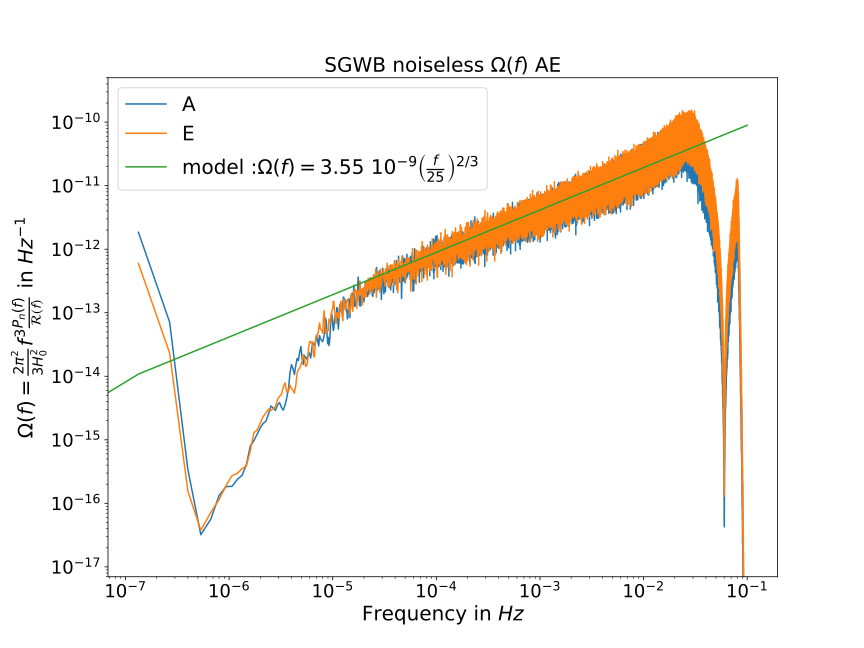
\includegraphics[width=1.\linewidth]{noiseless/Omega_AE}
  \caption{Total frequency band }
\end{subfigure}%
\begin{subfigure}{.5\textwidth}
  \centering
  \includegraphics[width=1.\linewidth]{noiseless/Omega_AET}
  \caption{Reduce frequency band [$2.15 \ 10^{-5}$, $9.98 \ 10^{-3}$] $\text{Hz}$}
\end{subfigure}
\caption{Channels [A,E] of the Spectral energy density of the stochastic Gravitational Wave Background from galactic foreground $\Omega_{GW}(f)$ of the MLDC for the noiseless channel.}
\label{fig:Omeganoiseless}
\end{figure}

\begin{figure}[H]
\begin{subfigure}{.5\textwidth}
  \centering
  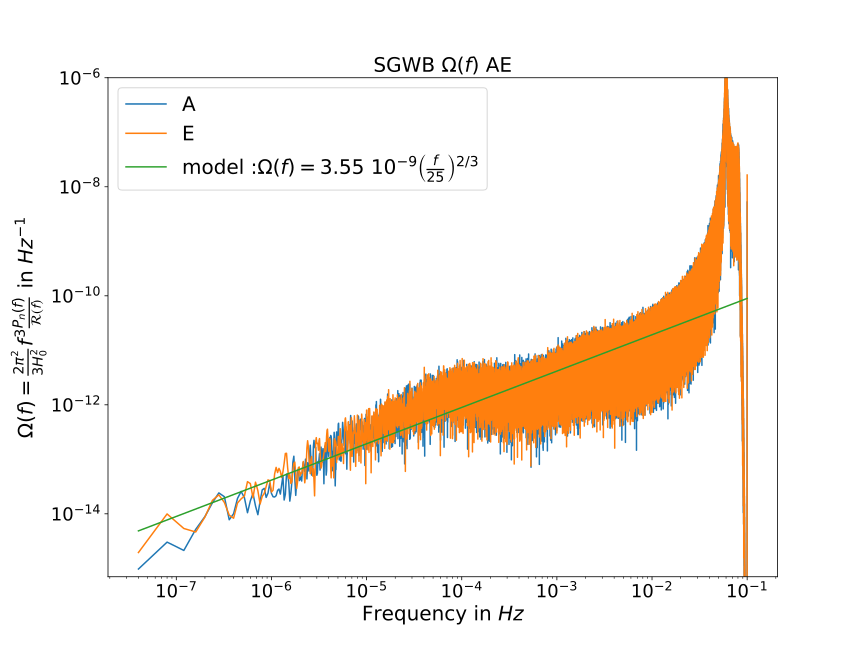
\includegraphics[width=1.\linewidth]{Omega_AE}
  \caption{Total frequency band }
  
\end{subfigure}%
\begin{subfigure}{.5\textwidth}
  \centering
  \includegraphics[width=1.\linewidth]{Omega_AET}
  \caption{Reduce frequency band $[2.15 \ 10^{-5}, \   9.98 \ 10^{-3}] \text{ Hz}$}
\end{subfigure}
\caption{Channels [A,E] of the Spectral energy density of the stochastic Gravitational Wave Background from galactic foreground $\Omega_{GW}(f)$ of the MLDC for the noisy channel.}
\label{fig:Omeganoisely}
\end{figure}

\subsection{Total simulation of the Stochastic Gravitational Wave Background (SGWB)}

To generate a full simulation of the Stochastic Gravitational Wave Background, a cosmological background should be added to the galactic foreground. The Cosmological Stochastic Gravitational Wave Background can be modeled by a second power law $\Omega_{GW,Cosmo} = \Omega_0 \left(\frac{f}{f_*}\right)^0$.  We have added to the Spectral density energy from the MLDC a Cosmological background $\Omega_0$ randomized with a Gaussian noise. We have created a background class of stochastic gravitational waves by varying the value of the cosmological background $\Omega_0 =$ [$1 \ 10^{-12}$, $2 \ 10^{-12}$, $5 \ 10^{-12}$, $1 \ 10^{-11}$, $2 \ 10^{-11}$, $5 \ 10^{-11}$, $1 \ 10^{-10}$, $2 \ 10^{-10}$, $5 \ 10^{-10}$, $1 \ 10^{-9}$, $2 \ 10^{-9}$, $5 \ 10^{-9}$, $1 \ 10^{-8}$] for the two channel $[A,E]$. The figure \ref{fig:Omega_tot} summarize the class of the simulation of the SGWB for the channel A, there is also the same class for the channel E. In the next, We chose to use noiseless Channels. In the thirteen tests, all the parameters except the cosmological amplitude are fixed. (We use $\Omega_{2/3} = 3.55 \ 10^{-9}$, $\alpha_{2/3}=2/3$ and $\alpha_{0o}=0$) Do generate the Data we use the model of the equation \ref{eq:Model}. We add to the MLDC foreground modeled by $\Omega_{GW,Astro}(f) = \Omega_{2/3} \left(\frac{f}{f_*}\right)^{2/3} +n(f)$ ($n(f)$ is a noise) and the $\Omega_{GW,Cosmo}(f) = \Omega_{0} \left(f\right)^{0}$ randomize with a normal distribution.

\begin{figure}[H]
    \centering
    \includegraphics[height= 7cm]{Omega_tot.png}
    \caption{Class of $13$ Spectral Energy density of the SGWB $\Omega_{GW}(f)$ of the channel A }
    \label{fig:Omega_tot}
\end{figure}


\section{Fitting of the Stochastic Gravitational Wave Background (SGWB) with Adaptive Makov chains Monte Carlo (A-McMC)}

In this section, we present the parametric estimation of the Stochastic Gravitational Wave Background with he method of Adaptive Makov chains Monte Carlo. We want to fit the model Eq~\ref{eq:Model} with the data of the class present in the figure \ref{fig:Omega_tot}.

\begin{equation}
\label{eq:Model}
	\Omega_{GW}(f) = \Omega_{GW,Astro}(f) + \Omega_{GW,Cosmo}(f) = \Omega_{2/3} \left(\frac{f}{f_*}\right)^{2/3} + \Omega_0 \left(\frac{f}{f_*}\right)^0
\end{equation}

\subsection{Setting of the Adaptive Markov chains Monte Carlo}

For a better fitting we chose to normalize the data from the class of simulation, we divide the Spectral Energy Density by the astrophysical gravitational wave amplitude $ \Omega_{2/3} = 3.55 \ 10^{-9}$.  It is obviously easier to fit parameters close to 1. For all the channel A,E and  Spectral Energy density Stochastic Gravitational Wave Background, we estimate 4 parameters : the normalize astrophysical gravitational wave amplitude $\overline{\Omega_{2/3}}$ the astrophysical slope $\alpha_{2/3}$, the normalize cosmological gravitational wave amplitude $\overline{\Omega_{0}}$ the astrophysical slope $\alpha_{0}$. We use the same frequency reference from the MLDC \cite{LDCM}, $f_* = 25 \ \text{Hz}$.The 26 Adaptive Markov chains Monte Carlo use 2 000 000 iterations for a duration for each estimation around 15h. In total, the estimation of all parametric estimation is 450 h. To perform the calculation we use the calculation center of the Observatoire de la Côte d'Azur, Licallo. In tables \ref{table:resultA} and \ref{table:resultE}, we present the 26 estimations of cosmological amplitude $\Omega_0 = \overline{\Omega_0}\Omega_{2/3} $.  

\begin{table}[H]
\begin{center}
\begin{tabular}{|l|l|l|}
\hline
Input $\Omega_0$    & Values of the McMC    & errors ($\sigma$)   \\ \hline
$1. \ 10^{-8}$      & $9.972 \ 10^{-9}$     & $8.97  \ 10^{-10}$  \\ \hline
$5. \ 10^{-9}$      & $4.986 \ 10^{-9}$     & $4.072 \ 10^{-10}$  \\ \hline
$2. \ 10^{-9}$      & $2.000 \ 10^{-9}$     & $1.463 \ 10^{-10}$  \\ \hline
$1. \ 10^{-9}$      & $1.018 \ 10^{-9}$     & $6.951 \ 10^{-11}$  \\ \hline
$5. \ 10^{-10}$     & $5.067 \ 10^{-10}$    & $3.201 \ 10^{-11}$  \\ \hline
$2. \ 10^{-10}$     & $2.101 \ 10^{-10}$    & $1.613 \ 10^{-11}$  \\ \hline
$1. \ 10^{-10}$     & $1.132 \ 10^{-10}$    & $1.713 \ 10^{-11}$  \\ \hline
$5. \ 10^{-11}$     & $5.507 \ 10^{-11}$    & $9.811 \ 10^{-12}$  \\ \hline
$2. \ 10^{-11}$     & $2.074 \ 10^{-11}$    & $6.990 \ 10^{-12}$  \\ \hline
$1. \ 10^{-11}$     & $1.050 \ 10^{-11}$    & $5.262 \ 10^{-12}$  \\ \hline
$5. \ 10^{-12}$     & $5.521 \ 10^{-12}$    & $2.568 \ 10^{-12}$  \\ \hline
$2. \ 10^{-12}$     & $2.525 \ 10^{-12}$    & $1.960 \ 10^{-12}$  \\ \hline
$1. \ 10^{-12}$     & $1.319 \ 10^{-12}$    & $9.976 \ 10^{-13}$  \\ \hline
\end{tabular}
\end{center}
\caption{Result of the A-McMC for the A channel}
\label{table:resultA}
\end{table}

\begin{table}[H]
\begin{center}
\begin{tabular}{|l|l|l|}
\hline
Input $\Omega_0$    & Values of the McMC    & errors ($\sigma$)   \\ \hline
$1. \ 10^{-8}$      & $1.039 \ 10^{-8}$     & $7.905 \ 10^{-10}$  \\ \hline
$5. \ 10^{-9}$      & $5.035 \ 10^{-9}$     & $4.098 \ 10^{-10}$  \\ \hline
$2. \ 10^{-9}$      & $1.990 \ 10^{-9}$     & $1.534 \ 10^{-10}$  \\ \hline
$1. \ 10^{-9}$      & $1.033 \ 10^{-9}$     & $8.752 \ 10^{-11}$  \\ \hline
$5. \ 10^{-10}$     & $5.184 \ 10^{-10}$    & $3.882 \ 10^{-11}$  \\ \hline
$2. \ 10^{-10}$     & $2.077 \ 10^{-10}$    & $1.315 \ 10^{-11}$  \\ \hline
$1. \ 10^{-10}$     & $1.096 \ 10^{-10}$    & $1.516 \ 10^{-11}$  \\ \hline
$5. \ 10^{-11}$     & $5.507 \ 10^{-11}$    & $9.811 \ 10^{-12}$  \\ \hline
$2. \ 10^{-11}$     & $2.175 \ 10^{-11}$    & $1.013 \ 10^{-11}$  \\ \hline
$1. \ 10^{-11}$     & $1.071 \ 10^{-11}$    & $3.943 \ 10^{-12}$  \\ \hline
$5. \ 10^{-12}$     & $4.286 \ 10^{-12}$    & $1.970 \ 10^{-12}$  \\ \hline
$2. \ 10^{-12}$     & $2.302 \ 10^{-12}$    & $2.074 \ 10^{-12}$  \\ \hline
$1. \ 10^{-12}$     & $2.345 \ 10^{-12}$    & $9.427 \ 10^{-13}$  \\ \hline
\end{tabular}
\end{center}
\caption{Result of the A-McMC for the E channel}
\label{table:resultE}
\end{table}

The figure \ref{fig:corner10} and the figure \ref{fig:corner12} are two results of the Adaptive-McMC of parametric estimation for respectively $ \Omega_0 = 1 \ 10^{-10} $ and $\Omega_0 = 1 \ 10^{-12}$. On this plot figure we can distinguished the posterior distribution of four estimate parameters, the posterior distribution from the histogram of the Markov chains, this is the distribution of an unknown quantity. In our case this distribution look-like normal distribution. 


\begin{figure}[H]
    \centering
    \includegraphics[height= 10cm]{1e-10/corners.png}
    \caption{Corner plot of the Adaptive-McMC of the channel A for a Cosmological Wave background amplitude of $\Omega_0 = 1,0 \ 10^{-10} $.  }
    \label{fig:corner10}
\end{figure}

\begin{figure}[H]
    \centering
    \includegraphics[height= 10cm]{corners.png}
    \caption{Corner plot of the Adaptive-McMC of the channel A for a Cosmological Wave background amplitude of $\Omega_0 = 1,0 \ 10^{-12} $. }
    \label{fig:corner12}
\end{figure}

\section{Fisher study of the separability and Adaptive Markov chains Monte Carlo} \label{sc:fisher+MCMC}

According to the section~\ref{study1}, we can have an estimation of the uncertainty of the estimation of parameter $\Omega_0$. The uncertainty is $\frac{\Delta \Omega_0}{\Omega_0}$. To estimate this quantity from the Fisher Information, we calculate the integral of the section \ref{spectral}    and the Inverse matrix of the Fisher Information (blue line on the figure \ref{fig:Fisher}). We can predict a better separability (uncertainty is less) for high value of the Cosmological background. The law level can be fit but with a high error (the error of the parameter and the estimation of the parameter will be near). 

The uncertainty can be calculated independently with the Adaptive-McMC calculation : 

\begin{equation}
\frac{\Delta \Omega_0}{\Omega_0} = \frac{\sigma_{\Omega_0}}{\Omega_0}
\end{equation}This ratio are the blue scatters for the channel A and the orange scatters for the channel E. We can estimate the errors of the uncertainty (from the McMC) for the channel I:

\begin{equation}
{Error}_{+,I} = \frac{\sigma_{\Omega_0}}{\left|\Omega_0-\sigma_{\Omega_0}\right|}
\end{equation}
\begin{equation}
{Error}_{-,I} = \frac{\sigma_{\Omega_0}}{\left|\Omega_0+\sigma_{\Omega_0}\right|}
\end{equation}Respectably we have in green the error bars for the channel A and for the channel E the error bars in red. The horizontal red line represent the error level $50\%$. In fact, above the line, the error is greater than $50\%$ and less than on the one below. The same goes for the orange line which represents a $10\%$ error.

\begin{figure}[H]
    \centering
    \includegraphics[height= 7cm]{Uncertanity.png}
    \caption{Uncertainty of the estimation of the parameter  $\Omega_0$ (The Spectral Energy Density of the Gravitational Wave from the Cosmological Stochastic Gravitational Wave Background) from the Fisher Information study in blue line and the parametric estimation from the Adaptive Markov chains Monte Carlo in blue scatters for the channel A and orange scatters for the channel E  }
    \label{fig:Fisher}
\end{figure}

According to the figure \ref{fig:Fisher}, we can separate the cosmological background from the astrophysical background with a magnitude distance of 1000. The importance is not the value of the background but the distance between the two backgrounds magnitude. For a distance of $ \frac{\Omega_{astro}}{\Omega_{Cosmo}} = 1410$, we have a fitting uncertainty of $39,4\%$. this is the limit measure. For a more important distance we can fit the cosmological background but with a high uncertainty. 


\section{Stochastic gravitational wave background fitting with Markov chains Monte-Carlo update with the channel T} \label{sc:cov}

The channel T can be add to a fitting model on the Power spectral density to have parametric estimation of a SGWB. In this section we considered two channel the channel T and the channel A. We assume have an evidence the noise and the signal or identical in the channel A and T. According to T.L Smith and R. R. Caldwell \cite{PhysRevD.100.104055}. We can simulate the LISA noise in frequency domain.

\begin{equation}
\left\{
\begin{array}{l}
    PSD_A = S_A + N_A \\
  PSD_T = N_T
\end{array}
\right.
\end{equation}
With $S_A(f) = \frac{3H_0^2}{4 \pi^2} \frac{\Omega_{GW,\alpha}\left(\frac{f}{f_{ref}}\right)^{\alpha}}{f^3}$,$f_{ref}=25 \ \text{Hz}$ , the noise components $N_A(f)$ and $N_T(f)$ can be write:

\begin{equation}
\left\{
\begin{array}{l}
    N_A = N_1 - N_2 \\
    N_T = N_1 + 2 N_2 
\end{array}
\right.
\end{equation}

with 
\begin{equation}
\left\{
\begin{array}{l}
    N_1(f) = \left(4 S_s(f) + 8\left( 1 + \cos^2\left(\frac{f}{f_*}\right)\right) S_a(f)\right)|W(f)|^2 \\
    N_2(f) = -\left(2 S_s(f) + 8 S_a(f)\right)\cos\left(\frac{f}{f_*}\right)|W(f)|^2
\end{array}
\right.
\end{equation}
with $W(f) = 1 - e^{-\frac{2if}{f_*}}$ and 
\begin{equation}
\left\{
\begin{array}{l}
    S_s(f) = N_{Pos} \\
    S_a(f) = \frac{N_{acc}}{(2 \pi f)^4}\left( 1 + \left(\frac{0.4 \text{ mHz}}{f} \right)^2 \right)
\end{array}
\right.
\end{equation}
The magnitude level of the LISA noise budget from the LISA Science Requirements Document \cite{LSR}, we use the acceleration noise $N_{acc} = 1.44 \ 10^{-48} \ \text{s}^{-4}\text{Hz}^{-1}$ and the optical path-length fluctuation $N_{Pos} = 3.6 \ 10^{-41} \ \text{Hz}^{-1}$. We can estimated the magnitude of noises on the Channel T, we level of the physical components on the two channel A and T are the same. It is very important to use the channel T to estimate the noise on the channel A. Thus one gains in precision when adjusting the parameters of the stochastic background. Furthermore, by considering a single substance, it is possible to parameterized an A-MCMC four parameter $\theta = (N_{acc},N_{Pos},\Omega_{GW\alpha},\alpha)$
We can calculate the Co-variance matrix:

\begin{equation}
    <PSD_I(f),PSD_J(f)> = \mathcal{C}_{I,J}(\theta,f)
\end{equation}
with $I,J = [A,T]$.

 \begin{equation}
     \mathcal{C}(\theta,f) =
     \left(
     \begin{array}{cc}
      %S_A + N_A & N_{A,T}  \\
      %N_{A,T} & N_T\\
      S_A + N_A & 0 \\
      0 & N_T\\
     \end{array}
     \right)
 \end{equation}
 
  \begin{equation}
     \mathcal{C}^{-1}(\theta) = K
     \left(
     \begin{array}{cc}
      N_T & 0\\%-N_{A,T}  \\
      0 & S_A + N_A\\
      %-N_{A,T} & S_A + N_A\\
     \end{array}
     \right)
 \end{equation}
 with $K(f_k) = det(\mathcal{C}) = \frac{1}{(S_A + N_A)N_T}$
% with $K(f_k) = det(\mathcal{C}) = \frac{1}{(S_A + N_A)N_T-N_{A,T}^2}$ and $N_{A,T} = \sqrt{N_AN_T}$
 
 We use the definition of the whittle likelihood from the review of N. J. Cornish and J. D. Romano \cite{Romano2017} the log-likelihood is :
 
 \begin{equation} 
\begin{split}
     %\mathcal{L}(\textbf{d}|\theta) & =  - \sum_{k=0}^N \Bigg[\frac{1}{4  K} \bigg(d_A(f_k)N_T(f_k) + \sqrt{d_A(f_k)d_T(f_k)}N_{A,T}(f_k)  \\ 
    %&+ d_T(f_k)\big(S_A(f_k) + N_A(f_k)\big) \bigg) + \ln\left(2\pi K(f_k) \right)\Bigg] 
          \mathcal{L}(\textbf{d}|\theta) & =  -\frac{1}{2} \sum_{k=0}^N \Bigg[ \sum_{I,J = [A,E,T]} \left( \sqrt{d_I(f)} \left(\mathcal{C}^{-1}\right)_{IJ} \sqrt{d_J(f)} \right)  + \ln\left(2\pi K(f_k) \right) \Bigg] \\
    &=  -\frac{1}{2} \sum_{k=0}^N \Bigg[ \frac{d_A^2}{S_A+N_A}   +\frac{d_T^2}{N_T} + \ln\left(8\pi^3 (S_A+NA)(S_E+N_E)N_T \right) \Bigg]  \Bigg] 
\end{split}
\end{equation}

\begin{equation} 
\begin{split}
    % F_{ab} & =   \frac{1}{2} \mathrm{Tr}\left(\mathcal{C}^{-1}\frac{\partial \mathcal{C}} {\partial \theta_a} \mathcal{C}^{-1} \frac{\partial \mathcal{C}}{\partial\theta_b}  \right)  \\ 
    % &=  \sum_{k=0}^{N} \frac{1}{2\left((S_A + N_A)N_T-N_{A,T}^2\right)^2}\\
    %&\Bigg[ \left(N_T \frac{\partial}{\partial \theta_a} (S_A + N_A) - \frac{1}{2}\frac{\partial}{\partial \theta_a}N_{A,T}^2 \right) \left(N_T \frac{\partial}{\partial \theta_b} (S_A + N_A) -\frac{1}{2}\frac{\partial}{\partial \theta_b}N_{A,T}^2 \right)\\
    %&- \left(N_T \frac{\partial}{\partial \theta_a} N_{A,T} + N_{A,T}\frac{\partial}{\partial \theta_a}(S_A + N_A) \right) \left(N_{A,T} \frac{\partial}{\partial \theta_b} (S_A + N_A)  + (S_A + N_A)\frac{\partial}{\partial \theta_b}N_{A,T} \right) \\
    %&-  \frac{\partial}{\partial \theta_a} \Big( (S_A + N_A)N_{A,T}\Big) \frac{\partial}{\partial \theta_b} \Big( (S_A + N_A)N_{A,T}\Big) \\
    %&+ \frac{1}{4}\left(\frac{\partial}{\partial \theta_a}N_{A,T}^2  + \frac{\partial}{\partial \theta_a}(S_A + N_A)^2 \right) \left(\frac{\partial}{\partial \theta_b}N_{A,T}^2  + \frac{\partial}{\partial \theta_b}(S_A + N_A)^2 \right)  \Bigg] 
     F_{ab} & =   \frac{1}{2} \mathrm{Tr}\left(\mathcal{C}^{-1}\frac{\partial \mathcal{C}} {\partial \theta_a} \mathcal{C}^{-1} \frac{\partial \mathcal{C}}{\partial\theta_b}  \right)  \\ 
     &=  \sum_{k=0}^{N} \Bigg[\frac{\frac{\partial (S_A+N_A)} {\partial \theta_a}\frac{\partial (S_A+N_A)} {\partial \theta_b}}{2(S_A+N_A)^2} + \frac{\frac{\partial N_T} {\partial \theta_a}\frac{\partial N_T} {\partial \theta_b}}{2N_T^2}\Bigg]
\end{split}
\end{equation}

If we have the channel T as zero and if we have a second science channel E, we obtain:
\begin{equation}
    F_{ab} =  \frac{1}{2} \sum_{I=A,E} \sum_{k=0}^N \frac{\frac{\partial S_I(f)+ N_I(f)} {\partial \theta_a}\frac{\partial S_I(f)+ N_I(f)} {\partial \theta_b}}{\left(S_a(f)+ N_a(f)\right)^2} 
\end{equation}

We have a comparing result given by \cite{PhysRevD.100.104055}, the inverse of the Fisher Information give on the diagonal the uncertainties of the estimation of the parameter. We see the importance to estimated the Sagnac (Channel T) for the estimation of the SGWB.  

\begin{figure}[H]
    \centering
    \includegraphics[height= 7cm]{covarince/Data+McMC.png}
    \caption{Power Spectral Density of the Channel A and T  from the LISA noise model \cite{PhysRevD.100.104055} and single SGWB. The top figure is the Power Spectral Density of the channel T and the bottom is the Power Spectral Density of the channel A with the parameter from the proposal \cite{LSR}. The orange line is the LISA noise model from \cite{PhysRevD.100.104055}  and in green the values fitted by the McMC and in grey the error at 1 $\sigma$. }
    \label{fig_covmcmc}
\end{figure}

On the figure \ref{fig_covmcmc}, blue line is the data with $\theta = \bigg(1.44 \ 10^{-48} \ \text{s}^{-4}\text{Hz}^{-1}$, $3.6 \ 10^{-41} \ \text{Hz}^{-1}$, $3.54 \ 10^{-9}$, $\frac{2}{3}\bigg)$(Orange line : model). The A-McMC is characterize by $\beta = 0.01$, $N = 1 \ 000 \ 000$ (see section~\ref{sec:adaptive}) and we use 2 000 parameter to estimate the co-variance matrice. We use log uniform prior with 10 magnitudes for the tree first parameters and a uniform prior for the slope between $-\frac{4}{3}$ and $\frac{8}{3}$. In green line the result of the A-McMC and in grey the error for 1 $\sigma$. The figure \ref{fig_corncovmcmc}, is the corner plot of the chains the posterior distribution are Gaussian. We have the evidence of a good fitting. The integration of the noise level magnitude on the parametric estimation is a success because we have the possibility to fit the background with the noise level with all the frequency domain, it is also possible to have a very efficient estimation of the different noise components thanks to the signal T devoid of 'science' source.


\begin{figure}[H]
    \centering
    \includegraphics[height= 7.5cm]{covarince/Corner.png}
    \caption{Corner plot of the Adaptive-McMC of the Power Spectral Density of the Channel A,T. Fitting of the two magnitude of the LISA noise model from Proposal \cite{LSR} and a single SGWB}
    \label{fig_corncovmcmc}
\end{figure}

We can also write a McMC with 6 parameters 2 for the noise Channel T, 2 for the astrophysical foreground and 2 for the cosmological background. To compare the result with the previous calculation with noise channel fitting estimation. We chose to calculate 13 Adaptive Markov chain Monte-Carlo (see Table \ref{table:resultA+T}) with different values of Cosmological Amplitude.  The A-McMC is characterize by $\beta = 0.01$, $N = 1 \ 000 \ 000$ (see section~\ref{sec:adaptive}) and we use 2 000 parameter to estimate the co-variance matrice. We use log uniform prior with 10 magnitudes for the 3 noise Channel parameters and the two background amplitudes and a uniform prior for the slope between $-0.4$ and $0.4$ for the cosmological slope and a uniform prior between $0.4$ and $0.9$ for the astrophysical slope. 

\begin{table}[H]
\begin{center}
\begin{tabular}{|l|l|l|}
\hline
Input $\Omega_0$    & Values of the McMC     & errors ($\sigma$)         \\ \hline
$1. \ 10^{-8}$      & $1.012 \ 10^{-08}$     & $9.108 \ 10^{-10}$   \\ \hline
$5. \ 10^{-9}$      & $4.773 \ 10^{-09}$     & $3.945 \ 10^{-10}$   \\ \hline
$2. \ 10^{-9}$      & $1.961 \ 10^{-09}$     & $1.730 \ 10^{-10}$   \\ \hline
$1. \ 10^{-9}$      & $9.833 \ 10^{-10}$     & $9.053 \ 10^{-11}$   \\ \hline
$5. \ 10^{-10}$     & $4.992 \ 10^{-10}$     & $5.353 \ 10^{-11}$   \\ \hline
$2. \ 10^{-10}$     & $2.001 \ 10^{-10}$     & $2.521 \ 10^{-11}$   \\ \hline
$1. \ 10^{-10}$     & $1.008 \ 10^{-10}$     & $1.448 \ 10^{-11}$   \\ \hline
$5. \ 10^{-11}$     & $5.157 \ 10^{-11}$     & $8.847 \ 10^{-12}$   \\ \hline
$2. \ 10^{-11}$     & $1.963 \ 10^{-11}$     & $3.926 \ 10^{-12}$   \\ \hline
$1. \ 10^{-11}$     & $1.012 \ 10^{-11}$     & $2.732 \ 10^{-12}$   \\ \hline
$5. \ 10^{-12}$     & $4.992 \ 10^{-12}$     & $1.997 \ 10^{-12}$   \\ \hline
$2. \ 10^{-12}$     & $1.932 \ 10^{-12}$     & $1.353 \ 10^{-12}$   \\ \hline
$1. \ 10^{-12}$     & $1.090 \ 10^{-12}$     & $1.145 \ 10^{-12}$   \\ \hline
\end{tabular}
\end{center}
\caption{Result of the A-McMC for the A channel with the channel T with $\Omega_{Astro} = 3.54 \ 10^{-9}$}
\label{table:resultA+T}
\end{table}

\begin{table}[H]
\begin{center}
\begin{tabular}{|l|l|l|}
\hline
Input $\Omega_0$    & Values of the McMC     & errors ($\sigma$)    \\ \hline
$1. \ 10^{-8}$      & $1.113 \ 10^{-08}$     & $1.067 \ 10^{-09}$   \\ \hline
$5. \ 10^{-9}$      & $4.875 \ 10^{-09}$     & $4.578 \ 10^{-10}$  \\ \hline
$2. \ 10^{-9}$      & $2.042 \ 10^{-09}$     & $2.028 \ 10^{-10}$   \\ \hline
$1. \ 10^{-9}$      & $9.936 \ 10^{-10}$     & $1.129 \ 10^{-10}$   \\ \hline
$5. \ 10^{-10}$     & $5.044 \ 10^{-10}$     & $7.473 \ 10^{-11}$   \\ \hline
$2. \ 10^{-10}$     & $2.015 \ 10^{-10}$     & $3.939 \ 10^{-11}$   \\ \hline
$1. \ 10^{-10}$     & $1.205 \ 10^{-10}$     & $3.191 \ 10^{-11}$   \\ \hline
$5. \ 10^{-11}$     & $4.937 \ 10^{-11}$     & $2.212 \ 10^{-11}$   \\ \hline
$2. \ 10^{-11}$     & $1.934 \ 10^{-11}$     & $1.233 \ 10^{-11}$   \\ \hline
$1. \ 10^{-11}$     & $9.947 \ 10^{-12}$     & $1.036 \ 10^{-11}$   \\ \hline
$5. \ 10^{-12}$     & $5.022 \ 10^{-12}$     & $8.480 \ 10^{-12}$   \\ \hline
$2. \ 10^{-12}$     & $2.013 \ 10^{-12}$     & $5.567 \ 10^{-12}$   \\ \hline
$1. \ 10^{-12}$     & $1.154 \ 10^{-12}$     & $5.508 \ 10^{-12}$   \\ \hline
\end{tabular}
\end{center}
\caption{Result of the A-McMC for the A channel with the channel T with $\Omega_{Astro} = 3.54 \ 10^{-8}$}
\label{table:resultA+T-8}
\end{table}

\begin{table}[H]
\begin{center}
\begin{tabular}{|l|l|l|}
\hline
Input $\Omega_0$    & Values of the McMC    & errors ($\sigma$)   \\ \hline
$1. \ 10^{-8}$      & $1.035 \ 10^{-08}$    & $9.313 \ 10^{-10}$  \\ \hline
$5. \ 10^{-9}$      & $5.075 \ 10^{-09}$    & $3.998 \ 10^{-10}$  \\ \hline
$2. \ 10^{-9}$      & $1.961 \ 10^{-09}$    & $1.691 \ 10^{-10}$  \\ \hline
$1. \ 10^{-9}$      & $1.031 \ 10^{-09}$    & $9.093 \ 10^{-11}$  \\ \hline
$5. \ 10^{-10}$     & $5.030 \ 10^{-10}$    & $5.311 \ 10^{-11}$  \\ \hline
$2. \ 10^{-10}$     & $2.091 \ 10^{-10}$    & $2.129 \ 10^{-11}$  \\ \hline
$1. \ 10^{-10}$     & $1.027 \ 10^{-10}$    & $1.104 \ 10^{-11}$  \\ \hline
$5. \ 10^{-11}$     & $5.081 \ 10^{-11}$    & $6.247 \ 10^{-12}$  \\ \hline
$2. \ 10^{-11}$     & $2.005 \ 10^{-11}$    & $2.406 \ 10^{-12}$  \\ \hline
$1. \ 10^{-11}$     & $1.111 \ 10^{-11}$    & $1.738 \ 10^{-12}$  \\ \hline
$5. \ 10^{-12}$     & $4.905 \ 10^{-12}$    & $9.293 \ 10^{-13}$  \\ \hline
$2. \ 10^{-12}$     & $2.043 \ 10^{-12}$    & $5.622 \ 10^{-13}$  \\ \hline
$1. \ 10^{-12}$     & $9.841 \ 10^{-13}$    & $2.953 \ 10^{-13}$  \\ \hline
\end{tabular}
\end{center}
\caption{Result of the A-McMC for the A channel with the channel T with $\Omega_{Astro} = 3.54 \ 10^{-10}$}
\label{table:resultA+T-10}
\end{table}

\begin{figure}[H]
    \centering
    \includegraphics[height= 8cm]{FisherAT/Fisherii.png}
    \caption{Evolution of Uncertainties of the estimation of the parameter $[\Omega_0, \alpha_0, \Omega_{2/3}, \alpha_{2/3}]$ versus the Cosmological amplitude $\Omega_0$. The precision measure of the parameter is affect by the value of the Cosmological amplitude $\Omega_0$.}
    \label{fig:FisheriiAE}
\end{figure}

\begin{figure}[H]
    \centering
    \includegraphics[height= 8cm]{FisherAT/Uncertanity2.png}
    \caption{Uncertainty of the estimation of the parameter $\Omega_0$ (The Spectral Energy Density of the Gravitational Wave from the Cosmological Stochastic Gravitational Wave Background) from the Fisher Information study in line (with the Cramer-Rao calculation) and the parametric estimation from the Adaptive Markov chains Monte Carlo in scatters for the channel A with the noise channel T. We chose to calculate the study with different value of Astrophysics magnitude $\Omega_{astro}$.   }
    \label{fig:Fisher2}
\end{figure}

According to the figure \ref{fig:Fisher2}, we can separate the cosmological background from the astrophysical background with a magnitude distance of 500. The importance is not the value of the background but the distance between the two backgrounds magnitude. If we considerate $\Omega_{astro} = 3.54 \ 10^{-9}$. For a distance of $ \frac{\Omega_{astro}}{\Omega_{Cosmo}} = 453$, we have a fitting uncertainty of $50\%$. this is the limit measure. For a more important distance we can fit the cosmological background but with a high uncertainty. In the figure \ref{fig:Fisher2}, this is the same study with three values of Astrophysical Background ($\Omega_{astro} = 3.54 \ 10^{-8}$, $3.54 \ 10^{-9}$ and $3.54 \ 10^{-10}$). The value of the McMC are in the tables \ref{table:resultA+T-8}, \ref{table:resultA+T} and \ref{table:resultA+T-10}. The figures \ref{fig:Corner6param} and \ref{fig:Corner6param2} are respectably  examples of a corner plot of Chains and posterior distribution for a run of 6 parameters Adaptive Markov chains Monte Carlo with $\Omega_{GW,Astro} = 3.55 \ 10^{-8}$ and  $\Omega_{GW,Cosmo} = 1 \ 10^{-10}$, $\Omega_{GW,Astro} = 3.55 \ 10^{-9}$ and  $\Omega_{GW,Cosmo} = 5 \ 10^{-12}$.  The important of this study is not the magnitude but the rate between the two Amplitude backgrounds $\frac{\Omega_{astro}}{\Omega_{Cosmo}}$. The rate is conserve for the background, but if we considerate the noise the time observation is important, according to the MLDC \cite{LDCM} the magnitude of the foreground ($3.54 \ 10^{-9}$) is given for 4 years of stacking. If, we observe during 10 year, we can imagine a factor 2.5 on the magnitude. On the figure \ref{fig:FisheriiAE}, we have the evidence of the influence of the precision on the fitting parameter versus the value of the Cosmological amplitude $\Omega_0$. Obviously, we understand that if the cosmological background is high it will be harder to measure the astrophysical background with great precision.

\begin{figure}[H]
    \centering
    \includegraphics[height= 16cm]{covarince/McMC6param/corners.png}
    \caption{Corner plot of the Chains and posterior distribution for a run of 6 parameters Adaptive Markov chains Monte Carlo, with $\Omega_{GW,Astro} = 3.55 \ 10^{-8}$ and  $\Omega_{GW,Cosmo} = 1 \ 10^{-10}$}
    \label{fig:Corner6param}
\end{figure}
\begin{figure}[H]
    \centering
    \includegraphics[height= 16cm]{covarince/McMC6param/corners2.png}
    \caption{Corner plot of the Chains and posterior distribution for a run of 6 parameters Adaptive Markov chains Monte Carlo, with $\Omega_{GW,Astro} = 3.55 \ 10^{-9}$ and  $\Omega_{GW,Cosmo} = 5 \ 10^{-12}$}
    \label{fig:Corner6param2}
\end{figure}

\section{Stochastic gravitational wave background fitting with Markov chains Monte-Carlo update with the channel T of the two "science" channels A and E}

The channel T can be add to a fitting model on the Power spectral density to have parametric estimation of a SGWB. In this section we considered two channel the channel T and the channel A. We assume have an evidence the noise and the signal or identical in the channel A and T. According to T.L Smith and R. R. Caldwell \href{https://arxiv.org/pdf/1908.00546.pdf}{PhysRevD.100.104055} \cite{PhysRevD.100.104055}. We can simulate the LISA noise in frequency domain.

\begin{equation}
\left\{
\begin{array}{l}
    PSD_A = S_A + N_A \\
    PSD_E = S_E + N_E \\
  PSD_T = N_T
\end{array}
\right.
\end{equation}
With $S_A(f) = S_E(f) =\frac{3H_0^2}{4 \pi^2} \frac{\Omega_{GW,\alpha}\left(\frac{f}{f_{ref}}\right)^{\alpha}}{f^3}$,$f_{ref}=25 \ \text{Hz}$ , the noise components $N_A(f)=N_E(f)$ and $N_T(f)$ can be write:

\begin{equation}
\left\{
\begin{array}{l}
    N_A = N_1 - N_2 \\
    N_T = N_1 + 2 N_2 
\end{array}
\right.
\end{equation}

with 
\begin{equation}
\left\{
\begin{array}{l}
    N_1(f) = \left(4 S_s(f) + 8\left( 1 + \cos^2\left(\frac{f}{f_*}\right)\right) S_a(f)\right)|W(f)|^2 \\
    N_2(f) = -\left(2 S_s(f) + 8 S_a(f)\right)\cos\left(\frac{f}{f_*}\right)|W(f)|^2
\end{array}
\right.
\end{equation}
with $W(f) = 1 - e^{-\frac{2if}{f_*}}$ and 
\begin{equation}
\left\{
\begin{array}{l}
    S_s(f) = N_{Pos} \\
    S_a(f) = \frac{N_{acc}}{(2 \pi f)^4}\left( 1 + \left(\frac{0.4 \text{ mHz}}{f} \right)^2 \right)
\end{array}
\right.
\end{equation}
The magnitude level of the LISA noise budget from the \href{https://atrium.in2p3.fr/nuxeo/nxdoc/default/f5a78d3e-9e19-47a5-aa11-51c81d370f5f/view_documents}{LISA Science Requirement}\cite{LSR} Document, we use the acceleration noise $N_{acc} = 1.44 \ 10^{-48} \ \text{s}^{-4}\text{Hz}^{-1}$ and the optical path-length fluctuation $N_{Pos} = 3.6 \ 10^{-41} \ \text{Hz}^{-1}$. We can estimated the magnitude of noises on the Channel T, we level of the physical components on the two channel A and T are the same. It is very important to use the channel T to estimate the noise on the channel A. Thus one gains in precision when adjusting the parameters of the stochastic background. Furthermore, by considering a single substance, it is possible to parameterized an A-MCMC eight parameters $\theta = (N_{acc},N_{Pos},A_1,\alpha_1, A_2, \alpha_2)$
We can calculate the Co-variance matrix:

\begin{equation}
    <PSD_I(f),PSD_J(f)> = \mathcal{C}_{I,J}(\theta,f) 
\end{equation}
with $I,J = [A,E,T]$.

 \begin{equation}
     \mathcal{C}(\theta,f) =
     \left(
     \begin{array}{ccc}
%      S_A + N_A & S_A + N_A & N_{A,T}  \\
%      S_A + N_A & S_A + N_A & N_{A,T}  \\
%      N_{A,T} & N_{A,T} & N_T\\
      S_A + N_A & 0 & 0  \\
      0 & S_E + N_E & 0 \\
      0 & 0 & N_T\\
     \end{array}
     \right)
 \end{equation}
 
  \begin{equation}
     \mathcal{C}^{-1}(\theta) = K
     \left(
     \begin{array}{ccc}
    %  -N_T & -N_T & 2N_{A,T}  \\
    %  -N_T & -N_T & 2N_{A,T}  \\
    %   2N_{A,T} & 2N_{A,T} & -4(S_A + N_A)\\
      (S_E+N_E)N_T & 0 & 0  \\
      0 & (S_A+N_A)N_T & 0  \\
      0 & 0 & (S_E+N_E)(S_A + N_A) \\
     \end{array}
     \right)
 \end{equation}
 with $K(f_k) = det(\mathcal{C}) = \frac{1}{(S_A + N_A)(S_E + N_E)N_T}$ %$K(f_k) = det(\mathcal{C}) = \frac{1}{N_{A,T}^2 - 4(S_A + N_A)N_T}$ and $N_{A,T} = \sqrt{N_AN_T}$
 
 We use the definition of the whittle likelihood from the review of N. J. Cornish and J. D. Romano \href{https://link.springer.com/content/pdf/10.1007/s41114-017-0004-1.pdf}{Romano2017} \cite{Romano2017} the log-likelihood is :
\begin{equation} 
\begin{split}
     \mathcal{L}(\textbf{d}|\theta) & =  -\frac{1}{2} \sum_{k=0}^N \Bigg[ \sum_{I,J = [A,E,T]} \left( \sqrt{d_I(f)} \left(\mathcal{C}^{-1}\right)_{IJ} \sqrt{d_J(f)} \right)  + \ln\left(2\pi K(f_k) \right) \Bigg] \\
    &=  -\frac{1}{2} \sum_{k=0}^N \Bigg[ \frac{d_A^2}{S_A+N_A}  + \frac{d_E^2}{S_E+N_E} + \frac{d_T^2}{N_T} +  \ln\left(8\pi^3 (S_A+NA)(S_E+N_E)N_T \right) \Bigg] 
\end{split}
\end{equation}

\begin{equation} 
\begin{split}
    % F_{ab} & =   \frac{1}{2} \mathrm{Tr}\left(\mathcal{C}^{-1}\frac{\partial \mathcal{C}} {\partial \theta_a} \mathcal{C}^{-1} \frac{\partial \mathcal{C}}{\partial\theta_b}  \right)  \\ 
    % &=  \sum_{k=0}^{N} \frac{8}{\left(4(S_A + N_A)N_T-N_{A,T}^2\right)^2}\\
    %&\Bigg\{ \frac{\partial}{\partial \theta_b} N_{A,T} \Bigg[(S_A + N_A)N_T \Bigg( N_T \frac{\partial}{\partial \theta_a} \left(\sqrt{\frac{N_A}{N_T}}\right) + (S_A + N_A)\frac{\partial}{\partial \theta_a}\left(\frac{N_{A,T}}{S_A + N_A}\right) \\
    %& + N_{A,T}\frac{\partial}{\partial \theta_a} \left(N_{A,T}^2-(S_A + N_A)N_T\right)   \Bigg)  \Bigg] \\
    %&-\frac{\partial}{\partial \theta_b} N_T \Bigg[ (S_A+N_A)^2 \left(  \frac{1}{2(S_A+N_A)} \frac{\partial}{\partial \theta_a} N_{A,T}^2 -\frac{\partial}{\partial \theta_a} N_{T} \right) \\ 
    %&+ N_{A,T}\frac{\partial}{\partial \theta_a}\left(\frac{N_{A,T}}{S_A + N_A}\right)\Bigg]\\
    %&+\frac{\partial}{\partial \theta_b} (S_A+N_A) \Bigg[ N_T \frac{\partial}{\partial \theta_a}(S_A + N_A) (N_T + 2N_{A,T}) \\
    %&-N_T \frac{\partial}{\partial \theta_a}\left( \frac{N_{A,T}^2}{2}\right) + N_{A,T}^2\frac{\partial}{\partial \theta_a}(N_T) \Bigg] \Bigg\}
     F_{ab} & =   \frac{1}{2} \mathrm{Tr}\left(\mathcal{C}^{-1}\frac{\partial \mathcal{C}} {\partial \theta_a} \mathcal{C}^{-1} \frac{\partial \mathcal{C}}{\partial\theta_b}  \right)  \\ 
     &=  \sum_{k=0}^{N} \Bigg[\frac{\frac{\partial (S_A+N_A)} {\partial \theta_a}\frac{\partial (S_A+N_A)} {\partial \theta_b}}{2(S_A+N_A)^2} + \frac{\frac{\partial (S_E+N_E)} {\partial \theta_a}\frac{\partial (S_E+N_E)} {\partial \theta_b}}{2(S_E+N_E)^2} + \frac{\frac{\partial N_T} {\partial \theta_a}\frac{\partial N_T} {\partial \theta_b}}{2N_T^2}\Bigg]
\end{split}
\end{equation}

If we have the channel T as zero and if we consider the two science channel A and E independent, we obtain:
\begin{equation}
    F_{ab} =  \frac{1}{2} \sum_{I=A,E} \sum_{k=0}^N \frac{\frac{\partial S_I(f)+ N_I(f)} {\partial \theta_a}\frac{\partial S_I(f)+ N_I(f)} {\partial \theta_b}}{\left(S_a(f)+ N_a(f)\right)^2} 
\end{equation}

We have a comparing result given by \cite{PhysRevD.100.104055}, the inverse of the Fisher Information give on the diagonal the uncertainties of the estimation of the parameter. We see the importance to estimated the Sagnac (Channel T) for the estimation of the SGWB.  

We can also write a McMC with 6 parameters 2 for the noise Channel T, 2 for the astrophysical foreground and 2 for the cosmological background with the two "science" channel. To compare the result with the previous calculation with noise channel fitting estimation. We chose to calculate 13 Adaptive Markov chain Monte-Carlo (see Table \ref{table:resultA+E+T}) with different values of Cosmological Amplitude.  The A-McMC is characterize by $\beta = 0.01$, $N = 4 \ 000 \ 000$ (see section~\ref{sec:adaptive}) and we use 2 000 parameter to estimate the co-variance matrice. We use log uniform prior with 10 magnitudes for the 3 noise Channel parameters and the two background amplitudes and a uniform prior for the slope between $-0.4$ and $0.4$ for the cosmological slope and a uniform prior between $0.27$ and $1.07$ for the astrophysical slope. 

\begin{table}[H]
\begin{center}
\begin{tabular}{|l|l|l|}
\hline
Input $\Omega_0$    & Values of the McMC     & errors ($\sigma$)    \\ \hline
$1. \ 10^{-8}$      & $1.069 \ 10^{-08}$     & $6.414 \ 10^{-10}$   \\ \hline
$5. \ 10^{-9}$      & $5.023 \ 10^{-09}$     & $3.013 \ 10^{-10}$   \\ \hline
$2. \ 10^{-9}$      & $1.979 \ 10^{-09}$     & $1.132 \ 10^{-10}$   \\ \hline
$1. \ 10^{-9}$      & $1.026 \ 10^{-09}$     & $1.132 \ 10^{-10}$   \\ \hline
$5. \ 10^{-10}$     & $5.087 \ 10^{-10}$     & $6.143 \ 10^{-11}$   \\ \hline
$2. \ 10^{-10}$     & $2.012 \ 10^{-10}$     & $3.195 \ 10^{-11}$   \\ \hline
$1. \ 10^{-10}$     & $1.031 \ 10^{-10}$     & $1.331 \ 10^{-11}$   \\ \hline
$5. \ 10^{-11}$     & $5.011 \ 10^{-11}$     & $8.240 \ 10^{-12}$   \\ \hline
$2. \ 10^{-11}$     & $2.002 \ 10^{-11}$     & $4.797 \ 10^{-12}$   \\ \hline
$1. \ 10^{-11}$     & $1.010 \ 10^{-11}$     & $3.009 \ 10^{-12}$   \\ \hline
$5. \ 10^{-12}$     & $5.008 \ 10^{-12}$     & $2.277 \ 10^{-12}$   \\ \hline
$2. \ 10^{-12}$     & $2.000 \ 10^{-12}$     & $1.661 \ 10^{-12}$   \\ \hline
$1. \ 10^{-12}$     & $1.048 \ 10^{-12}$     & $9.558 \ 10^{-13}$   \\ \hline
\end{tabular}
\end{center}
\caption{Result of the A-McMC for the A,E channel with the channel T with $\Omega_{Astro} = 3.54 \ 10^{-9}$}
\label{table:resultA+E+T}
\end{table}

\begin{table}[H]
\begin{center}
\begin{tabular}{|l|l|l|}
\hline
Input $\Omega_0$    & Values of the McMC     & errors ($\sigma$)    \\ \hline
$1. \ 10^{-8}$      & $1.033 \ 10^{-08}$     & $6.198 \ 10^{-10}$   \\ \hline
$5. \ 10^{-9}$      & $5.095 \ 10^{-09}$     & $3.057 \ 10^{-10}$   \\ \hline
$2. \ 10^{-9}$      & $1.988 \ 10^{-09}$     & $1.343 \ 10^{-10}$   \\ \hline
$1. \ 10^{-9}$      & $1.045 \ 10^{-09}$     & $6.947 \ 10^{-11}$   \\ \hline
$5. \ 10^{-10}$     & $5.012 \ 10^{-10}$     & $5.012 \ 10^{-11}$   \\ \hline
$2. \ 10^{-10}$     & $2.102 \ 10^{-10}$     & $3.153 \ 10^{-11}$   \\ \hline
$1. \ 10^{-10}$     & $1.016 \ 10^{-10}$     & $2.131 \ 10^{-11}$   \\ \hline
$5. \ 10^{-11}$     & $5.025 \ 10^{-11}$     & $1.558 \ 10^{-11}$   \\ \hline
$2. \ 10^{-11}$     & $2.050 \ 10^{-11}$     & $1.127 \ 10^{-11}$   \\ \hline
$1. \ 10^{-11}$     & $1.026 \ 10^{-11}$     & $1.093 \ 10^{-11}$   \\ \hline
$5. \ 10^{-12}$     & $5.030 \ 10^{-12}$     & $6.399 \ 10^{-12}$   \\ \hline
$2. \ 10^{-12}$     & $2.072 \ 10^{-12}$     & $5.822 \ 10^{-12}$   \\ \hline
$1. \ 10^{-12}$     & $1.006 \ 10^{-12}$     & $4.064 \ 10^{-12}$   \\ \hline
\end{tabular}
\end{center}
\caption{Result of the A-McMC for the A,E channel with the channel T with $\Omega_{Astro} = 3.54 \ 10^{-8}$}
\label{table:resultA+E+T-8}
\end{table}

\begin{table}[H]
\begin{center}
\begin{tabular}{|l|l|l|}
\hline
Input $\Omega_0$    & Values of the McMC    & errors ($\sigma$)   \\ \hline
$1. \ 10^{-8}$      & $1.030 \ 10^{-08}$    & $6.179 \ 10^{-10}$  \\ \hline
$5. \ 10^{-9}$      & $4.960 \ 10^{-09}$    & $2.976 \ 10^{-10}$  \\ \hline
$2. \ 10^{-9}$      & $2.056 \ 10^{-09}$    & $1.167 \ 10^{-10}$  \\ \hline
$1. \ 10^{-9}$      & $9.862 \ 10^{-10}$    & $5.769 \ 10^{-11}$  \\ \hline
$5. \ 10^{-10}$     & $5.019 \ 10^{-10}$    & $3.105 \ 10^{-11}$  \\ \hline
$2. \ 10^{-10}$     & $2.045 \ 10^{-10}$    & $1.351 \ 10^{-11}$  \\ \hline
$1. \ 10^{-10}$     & $1.048 \ 10^{-10}$    & $7.340 \ 10^{-12}$  \\ \hline
$5. \ 10^{-11}$     & $4.955 \ 10^{-11}$    & $3.715 \ 10^{-12}$  \\ \hline
$2. \ 10^{-11}$     & $2.006 \ 10^{-11}$    & $1.841 \ 10^{-12}$  \\ \hline
$1. \ 10^{-11}$     & $1.035 \ 10^{-11}$    & $1.001 \ 10^{-12}$  \\ \hline
$5. \ 10^{-12}$     & $5.033 \ 10^{-12}$    & $5.545 \ 10^{-13}$  \\ \hline
$2. \ 10^{-12}$     & $2.003 \ 10^{-12}$    & $2.667 \ 10^{-13}$  \\ \hline
$1. \ 10^{-12}$     & $1.062 \ 10^{-12}$    & $2.124 \ 10^{-13}$  \\ \hline
\end{tabular}
\end{center}
\caption{Result of the A-McMC for the A,E channel with the channel T with $\Omega_{Astro} = 3.54 \ 10^{-10}$}
\label{table:resultA+E+T-10}
\end{table}

\begin{figure}[H]
    \centering
    \includegraphics[height= 8cm]{FisherAET/Fisherii.png}
    \caption{Evolution of Uncertainties of the estimation of the parameter $[\Omega_0, \alpha_0, \Omega_{2/3}, \alpha_{2/3}]$ versus the Cosmological amplitude $\Omega_0$. The precision measure of the parameter is affect by the value of the Cosmological amplitude $\Omega_0$.}
    \label{fig:FisheriiAE}
\end{figure}

\begin{figure}[H]
    \centering
    \includegraphics[height= 8cm]{FisherAET/Uncertanity2.png}
    \caption{Uncertainty of the estimation of the parameter $\Omega_0$ (The Spectral Energy Density of the Gravitational Wave from the Cosmological Stochastic Gravitational Wave Background) from the Fisher Information study in line (with the Cramer-Rao calculation) and the parametric estimation from the Adaptive Markov chains Monte Carlo in scatters for the channel A with the noise channel T. We chose to calculate the study with different value of Astrophysics magnitude $\Omega_{astro}$.   }
    \label{fig:Fisher2}
\end{figure}

According to the figure \ref{fig:Fisher2}, we can separate the cosmological background from the astrophysical background with a magnitude distance of 500. The importance is not the value of the background but the distance between the two backgrounds magnitude. If we considerate $\Omega_{astro} = 3.54 \ 10^{-9}$. For a distance of $ \frac{\Omega_{astro}}{\Omega_{Cosmo}} = 453$, we have a fitting uncertainty of $50\%$. this is the limit measure. For a more important distance we can fit the cosmological background but with a high uncertainty. In the figure \ref{fig:Fisher2}, this is the same study with three values of Astrophysical Background ($\Omega_{astro} = 3.54 \ 10^{-8}$, $3.54 \ 10^{-9}$ and $3.54 \ 10^{-10}$). The value of the McMC are in the tables \ref{table:resultA+T-8}, \ref{table:resultA+T} and \ref{table:resultA+T-10}. The figures \ref{fig:Corner6param} and \ref{fig:Corner6param2} are respectably  examples of a corner plot of Chains and posterior distribution for a run of 6 parameters Adaptive Markov chains Monte Carlo with $\Omega_{GW,Astro} = 3.55 \ 10^{-8}$ and  $\Omega_{GW,Cosmo} = 1 \ 10^{-10}$, $\Omega_{GW,Astro} = 3.55 \ 10^{-9}$ and  $\Omega_{GW,Cosmo} = 5 \ 10^{-12}$.  The important of this study is not the magnitude but the rate between the two Amplitude backgrounds $\frac{\Omega_{astro}}{\Omega_{Cosmo}}$. The rate is conserve for the background, but if we considerate the noise the time observation is important, according to the MLDC \cite{LDCM} the magnitude of the foreground ($3.54 \ 10^{-9}$) is given for 4 years of stacking. If, we observe during 10 year, we can imagine a factor 2.5 on the magnitude. On the figure \ref{fig:FisheriiAE}, we have the evidence of the influence of the precision on the fitting parameter versus the value of the Cosmological amplitude $\Omega_0$. Obviously, we understand that if the cosmological background is high it will be harder to measure the astrophysical background with great precision.

\begin{figure}[H]
    \centering
    \includegraphics[height= 16cm]{FisherAET/1/corners.png}
    \caption{Corner plot of the Chains and posterior distribution for a run of 6 parameters Adaptive Markov chains Monte Carlo, with $\Omega_{GW,Astro} = 3.55 \ 10^{-8}$ and  $\Omega_{GW,Cosmo} = 1 \ 10^{-11}$}
    \label{fig:Corner6param}
\end{figure}
\begin{figure}[H]
    \centering
    \includegraphics[height= 16cm]{FisherAET/2/corners.png}
    \caption{Corner plot of the Chains and posterior distribution for a run of 6 parameters Adaptive Markov chains Monte Carlo, with $\Omega_{GW,Astro} = 3.55 \ 10^{-9}$ and  $\Omega_{GW,Cosmo} = 5 \ 10^{-12}$}
    \label{fig:Corner6param2}
\end{figure}

According to Parida et. al. \cite{2016JCAP...04..024P}, this is possible to detected the Isotropic Gravitational Wave Background. A method if the estimation of the amplitude of stochastic sources. The methods use the Maximum Likelihood parameter estimation with the Fisher Information matrices. primary the data need to be bias with noise model. We need to learn the slope of the different sources. A limit of this study is the variation of the background and this is difficult to use the channel T on the estimation of the Amplitude components in current knowledge of the method. This is also difficult to implement exotic model (not power law model). Indeed, recent work shows that the signal of astrophysical origin is not purely in law power.


\section{Conclusion}
In this paper we prove the evidence of the spectral separation of the two background with the Adaptive Markov chains Monte-Carlo method. We are also capable with a Fisher information study, predicting measurement uncertainty of the A-McMC. The two independent studies are coherent. This is an evidence of the possibility to separate the two components of the stochastic background. We obtained a uncertainty around 1 for the low level ($\Omega_0 = 1 \ 10^{-12}$) and around 0.03 for the high level ($\Omega_0 = 1 \ 10^{-8}$).
For example, with a astrophysical background of $\Omega_{GW,Astro} = 3.55 \ 10^{-9} \left(\frac{f}{25 \ \text{Hz}}\right)^{2/3}$ a cosmological background at $\Omega_{GW,Cosmo} = 6. \ 10^{-12}$ can be confident detect. It correspond to an uncertainty $\frac{\Delta \Omega_0 }{\Omega_0}$ of $0.5$ (red line in the figure~\ref{fig:Fisher}). The study from the section \ref{sc:fisher+MCMC} prove the possibility to fits the parametric components of the SGWB but we have to subtract the noise before and we have to reduce the frequency domain. In the section \ref{sc:cov}, we discus and prove the possibility to add the 'noise' channel (The channel $T$) to fit the magnitude noise components of the LISA noise budget. The advantage is to increase the efficiency of the fitting and have the total frequency domain $[1 \ 10^{-5} \ \text{Hz}, 1 \ \text{Hz}]$. We also calculate the new Fisher information study with the LISA noise. According to the figure \ref{fig:Fisher2} we prove the posibility to separate the two background with a spectral separation with a factor of $500$.       
%specify the (f/25 Hz)^(2/3) for the astro background. And for the cosmo background of 6 10^{-12}, state what \Delta \Omega/\Omega this corresponds to. 
\bibliographystyle{abbrv}
\bibliography{biblio}
\end{document}



